\documentclass[english,xcolor=svgnames]{beamer}


\usepackage{mathptmx}
\usepackage[OT1]{fontenc}
% \usepackage[latin9]{inputenc}
\usepackage{amsmath}
\usepackage{amssymb}
\usepackage{amsthm}
\usepackage{mathrsfs}
\usepackage{amsfonts}
\usepackage{eurosym}
\usepackage{bm}

\usepackage{booktabs}
\usepackage{tabularx}
\usepackage{subcaption}
\usepackage[makeroom,thicklines]{cancel}

\usepackage{multirow}
\usepackage{rotating}
\usepackage{array}
\usepackage{float}



\makeatletter

 \newcommand\makebeamertitle{\frame{\maketitle}}%
 \AtBeginDocument{
   \let\origtableofcontents=\tableofcontents
 \def\tableofcontents{\@ifnextchar[{\origtableofcontents}{\gobbletableofcontents}}
   \def\gobbletableofcontents#1{\origtableofcontents}
 }
 
 \usetheme{Boadilla}
\setbeamertemplate{footline}[frame number]{}
\usefonttheme{structuresmallcapsserif}
\setbeamercolor{title}{fg=blue}
\setbeamercolor{frametitle}{fg=blue}
\setbeamercolor{caption name}{fg=blue}
\setbeamercovered{transparent}


\beamertemplatenavigationsymbolsempty

\usepackage{booktabs}
\usepackage{tabularx}
\renewcommand{\tabularxcolumn}[1]{>{\centering\arraybackslash}m{#1}}
%\newcolumntype{L}{>{\centering}X}
%\newcolumntype{H}{>{\lrbox0}c<{\endlrbox}@{}}

%\let\estinput=\input
%\newcommand{\estwide}[3]{
%          \vspace{.75ex}{
%               \begin{tabularx}
%               {\textwidth}{@{\hskip\tabcolsep\extracolsep\fill}l*{#2}{#3}}
%               \toprule
%               \estinput{#1}
%               \bottomrule
%               \addlinespace[.75ex]
%               \end{tabularx}
%               }
%          }
%
%		\newcommand{\figtext}[1]{
%		     %\vspace{-1.9ex}
%		     \captionsetup{justification=justified,font=footnotesize}
%		     \caption*{\hspace{6pt}\hangindent=1.5em #1}
%		     }
%		\newcommand{\fignote}[1]{\figtext{\emph{Note:~}~#1}}
%
\usepackage{collcell}
%\makeatother
% \newcolumntype{G}{>{\collectcell\@gobble}c<{\endcollectcell}@{}}
% \makeatother
% \def\eatcell#1\unskip{}
% \newcolumntype{E}{>{\eatcell}c@{}}
%\usepackage{tabulary}
%\usepackage{multirow}
%\usepackage{dcolumn}
%\usepackage{pdflscape}
%\usepackage{pdfpages}
% \usepackage{epsfig}
% \usepackage{epstopdf}
% \usepackage{eso-pic}
\usepackage{graphicx}
%\usepackage{arydshln}
\usepackage[compatibility=false,font={sc,rm,color=blue},justification=centering,labelformat=empty, textfont=Large, margin=2pt]{caption}
\captionsetup[figure]{belowskip=0pt}

\newcommand{\rot}[2]{\rule{1em}{0pt}%
\makebox[0cm][c]{\rotatebox{#1}{\ #2}}}

\usepackage{siunitx} %For aligning decimals
\sisetup{ detect-mode, 
          group-digits            = false ,
          input-signs             = ,
          input-symbols           = ()[]-+* ,
          input-open-uncertainty  = ,
          input-close-uncertainty = ,
          table-align-text-post   = false, 
          table-number-alignment = center
}
\selectcolormodel{cmyk}
\usepackage{color,soul}
\usepackage{colortbl}
\usepackage{tikz}
\usetikzlibrary{matrix,shapes,arrows,intersections,calc}
\usepackage{verbatim}
\setbeamercovered{invisible}
\setbeamercolor{math text displayed}{fg=blue}
\setbeamercolor{math text inlined}{fg=blue}

%\let\olditem\item
%\renewcommand{\item}{\setlength{\itemsep}{\fill}\olditem}
\AtBeginDocument{\setlength\belowdisplayskip{0pt}}


\usepackage[english]{babel}
\usepackage{booktabs}
\usepackage{tablefootnote}
\usepackage{calc,hhline,ifthen,lscape} 

%\usepackage{enumitem}
%\let\olditem\item
%\renewcommand{\item}{\setlength{\itemsep}{\fill}\olditem}

% new math commands
\newcommand{\E}{\mathbb{E}}

\newcommand{\sym}[1]{\rlap{$#1$}} %For sym in STATA tables

\setbeamertemplate{frametitle}[default][center]

% \makeglossaries
% 
% \usepackage{pgfpages}
% \pgfpagesuselayout{resize to}[a4paper, landscape, border shrink=5mm]
\usepackage[absolute,overlay]{textpos}

\usepackage{epstopdf}


%\setlength{\itemsep}{\fill}



% ===========================================================
% ===========================================================
% ===========================================================
% Improves spacing of itemize and enumerate environment

\makeatletter
\renewcommand{\itemize}[1][]{%
  \beamer@ifempty{#1}{}{\def\beamer@defaultospec{#1}}%
  \ifnum \@itemdepth >2\relax\@toodeep\else
    \advance\@itemdepth\@ne
    \beamer@computepref\@itemdepth% sets \beameritemnestingprefix
    \usebeamerfont{itemize/enumerate \beameritemnestingprefix body}%
    \usebeamercolor[fg]{itemize/enumerate \beameritemnestingprefix body}%
    \usebeamertemplate{itemize/enumerate \beameritemnestingprefix body begin}%
    \list
      {\usebeamertemplate{itemize \beameritemnestingprefix item}}
      {\def\makelabel##1{%
          {%
            \hss\llap{{%
                \usebeamerfont*{itemize \beameritemnestingprefix item}%
                \usebeamercolor[fg]{itemize \beameritemnestingprefix item}##1}}%
          }%
        }%
      }
  \fi%
  \setlength\itemsep{\fill}
    \ifnum \@itemdepth >1
        \vfill
    \fi%  
  \beamer@cramped%
  \raggedright%
  \beamer@firstlineitemizeunskip%
}

\def\enditemize{\ifhmode\unskip\fi\endlist%
  \usebeamertemplate{itemize/enumerate \beameritemnestingprefix body end}
  \ifnum \@itemdepth >1
        \vfil
  \fi%  
  }
\makeatother


\makeatletter
\def\enumerate{%
	\ifnum\@enumdepth>2\relax\@toodeep
	\else%
	\advance\@enumdepth\@ne%
	\edef\@enumctr{enum\romannumeral\the\@enumdepth}%
	\advance\@itemdepth\@ne%
	\fi%
	\beamer@computepref\@enumdepth% sets \beameritemnestingprefix
	\edef\beamer@enumtempl{enumerate \beameritemnestingprefix item}%
	\@ifnextchar[{\beamer@@enum@}{\beamer@enum@}}
\def\beamer@@enum@[{\@ifnextchar<{\beamer@enumdefault[}{\beamer@@@enum@[}}
\def\beamer@enumdefault[#1]{\def\beamer@defaultospec{#1}%
	\@ifnextchar[{\beamer@@@enum@}{\beamer@enum@}}
\def\beamer@@@enum@[#1]{% partly copied from enumerate.sty
	\@enLab{}\let\@enThe\@enQmark
	\@enloop#1\@enum@
	\ifx\@enThe\@enQmark\@warning{The counter will not be printed.%
		^^J\space\@spaces\@spaces\@spaces The label is: \the\@enLab}\fi
	\def\insertenumlabel{\the\@enLab}
	\def\beamer@enumtempl{enumerate mini template}%
	\expandafter\let\csname the\@enumctr\endcsname\@enThe
	\csname c@\@enumctr\endcsname7
	\expandafter\settowidth
	\csname leftmargin\romannumeral\@enumdepth\endcsname
	{\the\@enLab\hspace{\labelsep}}%
	\beamer@enum@}
\def\beamer@enum@{%
	\beamer@computepref\@itemdepth% sets \beameritemnestingprefix
	\usebeamerfont{itemize/enumerate \beameritemnestingprefix body}%
	\usebeamercolor[fg]{itemize/enumerate \beameritemnestingprefix body}%
	\usebeamertemplate{itemize/enumerate \beameritemnestingprefix body begin}%
	\expandafter
	\list
	{\usebeamertemplate{\beamer@enumtempl}}
	{\usecounter\@enumctr%
		\def\makelabel##1{{\hss\llap{{%
						\usebeamerfont*{enumerate \beameritemnestingprefix item}%
						\usebeamercolor[fg]{enumerate \beameritemnestingprefix item}##1}}}}}%
	\setlength\itemsep{\fill}
	\ifnum \@itemdepth >1
	\vfill
	\fi%  
	\beamer@cramped%
	\raggedright%
	\beamer@firstlineitemizeunskip%
}
\def\endenumerate{\ifhmode\unskip\fi\endlist%
	\usebeamertemplate{itemize/enumerate \beameritemnestingprefix body end}
	\ifnum \@itemdepth >1
	\vfil
	\fi%  
}
\makeatother

% ===========================================================
% ===========================================================
% ===========================================================


%\usepackage[colorlinks=true]{hyperref}

\hypersetup{colorlinks = true,linkcolor = blue, bookmarksopen=true, bookmarksopenlevel=1}

%\hypersetup{bookmarksopen=true, bookmarksopenlevel=1}



\begin{document}

\title{Firm Aggregation}
\vspace{1cm}
\author[shortname]{
\begin{tabular}{cc}
Juan Herre\~{n}o & Johannes Wieland \\ 
\end{tabular}\\
}



\date{UCSD, Spring \the\year}

\setbeamertemplate{footline}{}
\makebeamertitle
\setbeamertemplate{footline}[frame number]{}

\addtocounter{framenumber}{-1}

%%%%%%%%%%%%%%%%%%%%%%%%%%%%%%%%%%%%%%%%%%%%%%%%%%
\AtBeginSection[]{
\setbeamertemplate{footline}{}
  \frame<beamer>{ 

    \frametitle{Outline}   

    \tableofcontents[currentsection,hideallsubsections] 
  }
\setbeamertemplate{footline}[frame number]{}
\addtocounter{framenumber}{-1}
}

\AtBeginSubsection[]{
\setbeamertemplate{footline}{}
  \frame<beamer>{ 

    \frametitle{Outline}   

    \tableofcontents[currentsection,currentsubsection] 
  }
  \setbeamertemplate{footline}[frame number]{}
  \addtocounter{framenumber}{-1}
}



\setbeamertemplate{footline}{}
\begin{frame}
\frametitle{Outline}   
\tableofcontents[hideallsubsections] 
\end{frame}
\addtocounter{framenumber}{-1}
\setbeamertemplate{footline}[frame number]{}

\section{The problem}

\begin{frame}{Many possibilities}
\begin{itemize}
\item Look at researchers you admire/know
\item They look at the same question from different perspectives
\item Evaluate evidence using a model / Evaluate a model using evidence
\item Personally, I need to write things down understand them
\item So I usually have model' in my work
\item Advice: Make notes, like lecture notes. You can avoid reinventing the wheel over and over again.
\item Don't derive the same Phillips curve 47 times in your career, have the notes somewhere.
\end{itemize}
\end{frame}

\begin{frame}{Goal}
Interested in estimating the effects of credit supply shocks
\begin{itemize}
\item If credit becomes scarce
\item Or more expensive
\item What happens to real economic activity?
\item Difficult to answer in the time series: severe reverse causality concerns
\item Bernanke 1983 is a fantastic read
\end{itemize}
\end{frame}

\begin{frame}{Illustration}
\begin{itemize}
\item Imagine a firm that ``needs financing''
\item Firms must finance expenditures in advance
$$TC_j = W N_j R_{j}$$
\item Total Loans $L_j$
$$L_j = W N_j$$
\item Assume the firm uses only labor
$$Y_j = A_j N_j$$
\item So the firm marginal cost is
$$ MC_j =  \frac{W R_j}{A_j}$$
\end{itemize}
\end{frame}

\begin{frame}{Illustration}
\begin{itemize}
\item Assume firms are monopolistic competitors
$$P_j = \frac{\eta}{\eta - 1} MC_j$$
\item And face a demand curve
$$Y_j = Y P_j^{-\eta}$$
\item Yielding 
$$Y_j = Y \left(\frac{\eta}{\eta - 1} \frac{WR_j}{A_j}\right)^{-\eta}$$
\item Or in logs

$$\log Y_j = -\eta \log R_j +  \eta \log A_j - \eta \log (\mu) + \log Y  - \eta \log W$$
\end{itemize}
\end{frame}

\begin{frame}{Illustration}
$$\log Y_j = -\eta \log R_j +  \eta \log A_j - \eta \log (\mu) + \log Y  - \eta \log W$$
\begin{itemize}
\item Take temporal differences
$$\Delta \log Y_j = -\eta\Delta \log R_j +  \eta \Delta  \log A_j  + \Delta \log Y  - \eta \Delta \log W$$
\item Assume that there are there are $N$ banks. Firms use only 1 (so $R_j$ is the $R$ of the bank firm $j$ uses).
\item Run a simple regression (do not observe $A$)
$$\Delta \log Y_j = \beta_0 + \beta_1 \Delta \log R_j  + \epsilon_j $$
\end{itemize}
\end{frame}

\begin{frame}{Illustration}
$$\Delta \log Y_j = \beta_0 + \beta_1 \Delta \log R_j  + \epsilon_j $$
What could be wrong?
\begin{itemize}
\item Remember our identifying assumption
$$\mathbb{E}(\Delta \log R_j \Delta \log A_j) = 0$$
\item In words: Shocks to banks are uncorrelated to the shocks of firms a bank lends to.
\item Things you are worried
\begin{itemize}
\item Reverse causality: Credit demand shocks: shock to the oil sector. Oil companies suffer. They reduce their borrowing from The First Oil Bank of America.
\item OVB I: A bank that lends to firms in construction, also holds mortgages in their assets. Housing bubble bursts.
\item OVB II : Local bank lends to local firms. There is a local demand shock. Banks deposits suffer. Firm demand suffers.
\end{itemize}
\end{itemize}
\end{frame}

\begin{frame}{Illustration}
Solution: Firm assignment as good as random.
\begin{itemize}
\item  Easier said that done
\end{itemize}
\end{frame}

\begin{frame}{Illustration}
\begin{itemize}
\item It is useful to think on a 2 x 2 dif-in-dif.
\item  Two banks, $G$ or $B$. $\bar{X}_i$ is the average of $X$ for firms that have bank $i$
$$\Delta \log \bar{Y}_B -\Delta  \log \bar{Y}_G = -\eta \left( \Delta  \log R_B - \Delta  \log R_G\right)  + \eta\left( \Delta \log \bar{A}_B - \Delta \log \bar{A}_G\right)$$
\item Covariance of $\Delta A$ and $\Delta R$ will dictate extent of bias
\item Aggregate variables drop out(soaked up in $\beta_0$. Missing intercept)
\item Elasticity being $\eta$ the result of many assumptions
\item In general, $\eta$ is not the aggregate effect
\end{itemize}
\end{frame}

\section{Khwaja and Mian 2008}
\begin{frame}{Khwaja and Mian 2008}
\begin{itemize}
\item Context: Nuclear tests in Pakistan in 1998
\item Government stopped USD deposit convertibility
\item Note: Not unusual. The American banking system suspended convertibility several times in the XIX and early XX century
\item The key references on bank runs and suspension of convertibility are
\begin{itemize}
\item Bryant 1980
\item Diamond Dybvig 1983
\item Gorton 1985
\end{itemize}
\end{itemize}
\end{frame}


\begin{frame}{Khwaja and Mian 2008}
\begin{itemize}
\item USD deposits widely popular
\item But heterogeneous across banks. Not random.
\item Firms deposited dollars in a commercial bank. Commercial banks sent the dollars to the CB in exchange for rupees. When a depositor demanded their deposits back, the CB handed the dollars to the commercial bank at the \textit{time of deposit} exchange rate.
\item Government allowed demand deposits back at the current (worse) exchange rate
\item Partial default on dollar deposits
\item Savers lost confidence and demanded their deposits back. Differential liquidity shock to the banks
\end{itemize}
\end{frame}

\begin{frame}{Khwaja and Mian 2008}
\begin{figure}
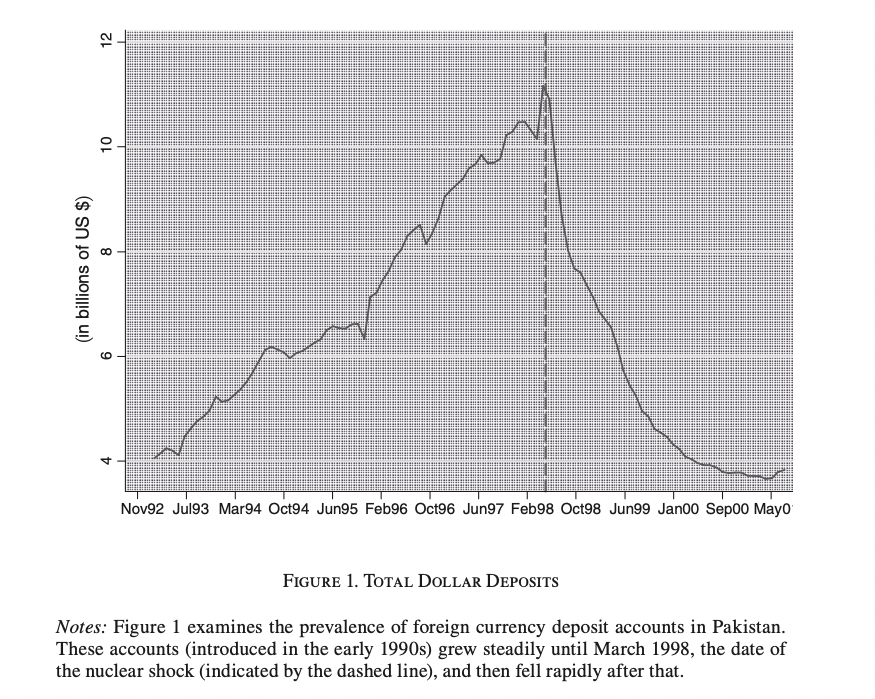
\includegraphics[scale=0.35]{figures/km_1}
\end{figure}
\end{frame}


\begin{frame}{Khwaja and Mian 2008}
\begin{figure}
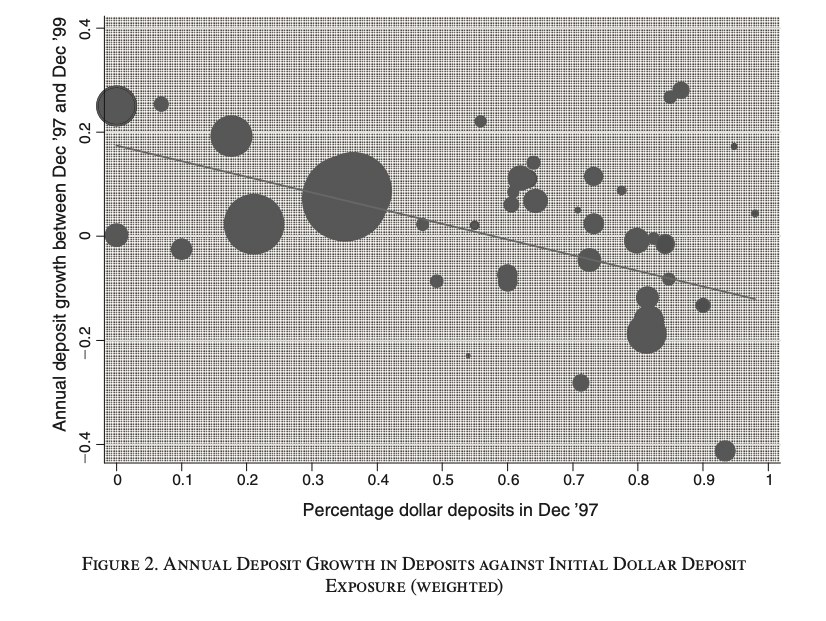
\includegraphics[scale=0.35]{figures/km_2}
\end{figure}
\end{frame}


\begin{frame}{Empirical Specification}
$$\Delta L_{ij} = \beta_j + \beta_1 \Delta D_i + \epsilon_{ij}$$
\begin{itemize}
\item $L_{ij}$ loan size of a firm-bank pair
\item $\beta_j$ firm fixed effect
\item $\Delta D_i$ change in bank-level dollar-denominated deposits
\item This firm-fixed effect approach became the standard in the literature
\end{itemize}
\end{frame}

\begin{frame}{Empirical Specification}
\begin{itemize}
\item Effectively uses only multi-bank firms
\item The firm fixed effect soaks any shock that causes changes in overall firm credit
\item How much firms increase their borrowing from one bank relative to another bank
\item What could go wrong?
\end{itemize}
\end{frame}

\begin{frame}{The null hypothesis}
$$\Delta L_{ij} = \beta_j + \beta_1 \Delta D_i + \epsilon_{ij}$$
\begin{itemize}
\item What is the economic meaning of the null hypothesis $H_0 : \beta_1 = 0$?
\item Think of two worlds in which $\beta_1 = 0$. Thoughts?
\end{itemize}
\end{frame}

\begin{frame}{Identifying assumption}
\begin{itemize}
\item Recall
$$\Delta L_{ij} = \beta_j + \beta_1 \Delta D_i + \epsilon_{ij}$$
\item What we need to assume
$$\mathbb{E}(\Delta D_i  \epsilon_{ij}) = 0$$
\item What does it mean?
\item Construct a scenario that breaks the assumption
\end{itemize}
\end{frame}

\begin{frame}{Results}
\begin{figure}
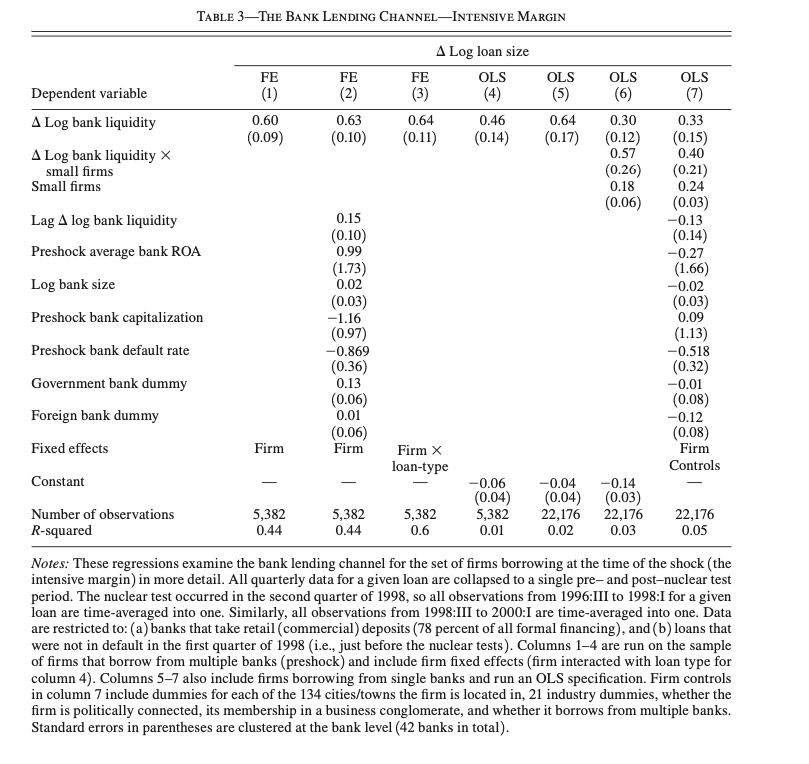
\includegraphics[scale=0.3]{figures/km_3}
\end{figure}\end{frame}


\begin{frame}{Results}
\begin{figure}
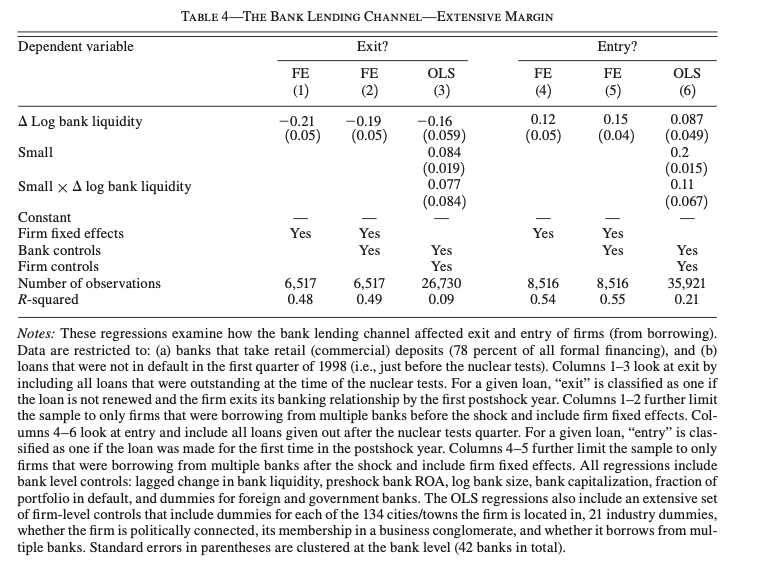
\includegraphics[scale=0.35]{figures/km_4}
\end{figure}
\end{frame}


\section{Chodorow-Reich 2014}

\begin{frame}{Motivation}
\begin{itemize}
\item Khwaja-Mian (2008) mostly about financial variables
\item In particular credit demand
\item Need variation within the firm
\item But are credit effects relevant at the firm level?
\item Aggregate bank-firm results at the firm level
\end{itemize}
\end{frame}


\begin{frame}{Ideal Regressor}
\begin{itemize}
\item Ideally, you would like the cost of capital of the bank
\item Difficult (impossible?) to observe
\item Uses an exposure measure instead
\item $L_{b,j,t}$ The loans given by bank $b$ to firm $j$ in period $t$
\item Change in bank credit
$$\Delta L_{-i,b} = \frac{\sum_{i \neq j} \alpha_{b,j,crisis} L_{b,j,crisis}}{\sum_{i \neq j} \alpha_{b,j,normal} L_{b,j,normal}}$$
\item Exposure measure
$$\Delta \tilde{L}_{i,s} = \sum_{b \in s} \alpha_{b,i,last} \Delta L_{-i,b}$$
\item Shift-share. Bank-level shocks, firm-level exposure
\item Exogenous shifts? Exogenous shares?
\end{itemize}
\end{frame}


\begin{frame}{Firm-bank relationships are sticky}
\begin{figure}
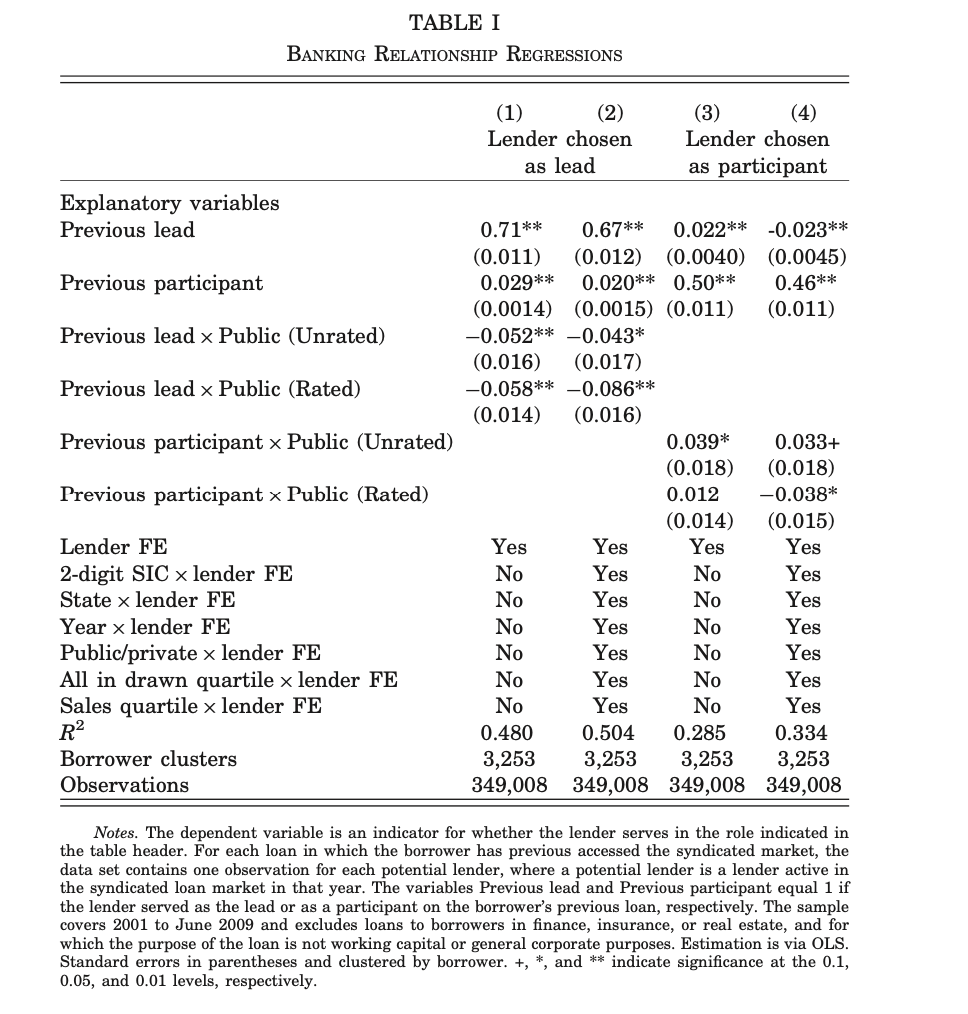
\includegraphics[scale=0.45]{figures/cr_1}
\end{figure}
\end{frame}

\begin{frame}{IV First Stage}
\begin{figure}
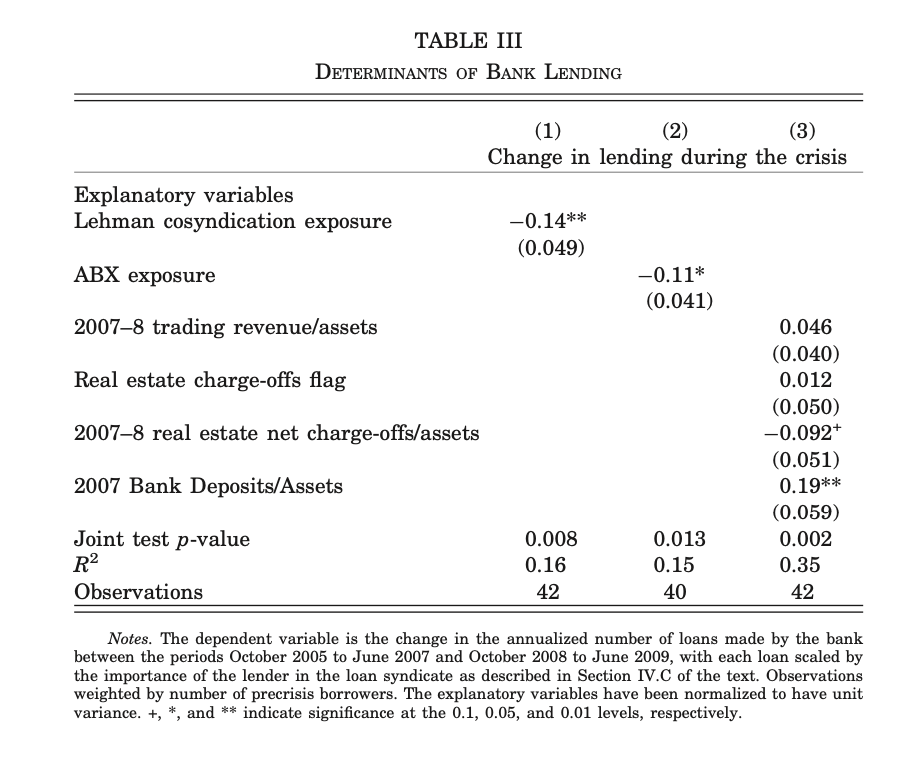
\includegraphics[scale=0.45]{figures/cr_2}
\end{figure}
\end{frame}


\begin{frame}{Results on Rates}
\begin{figure}
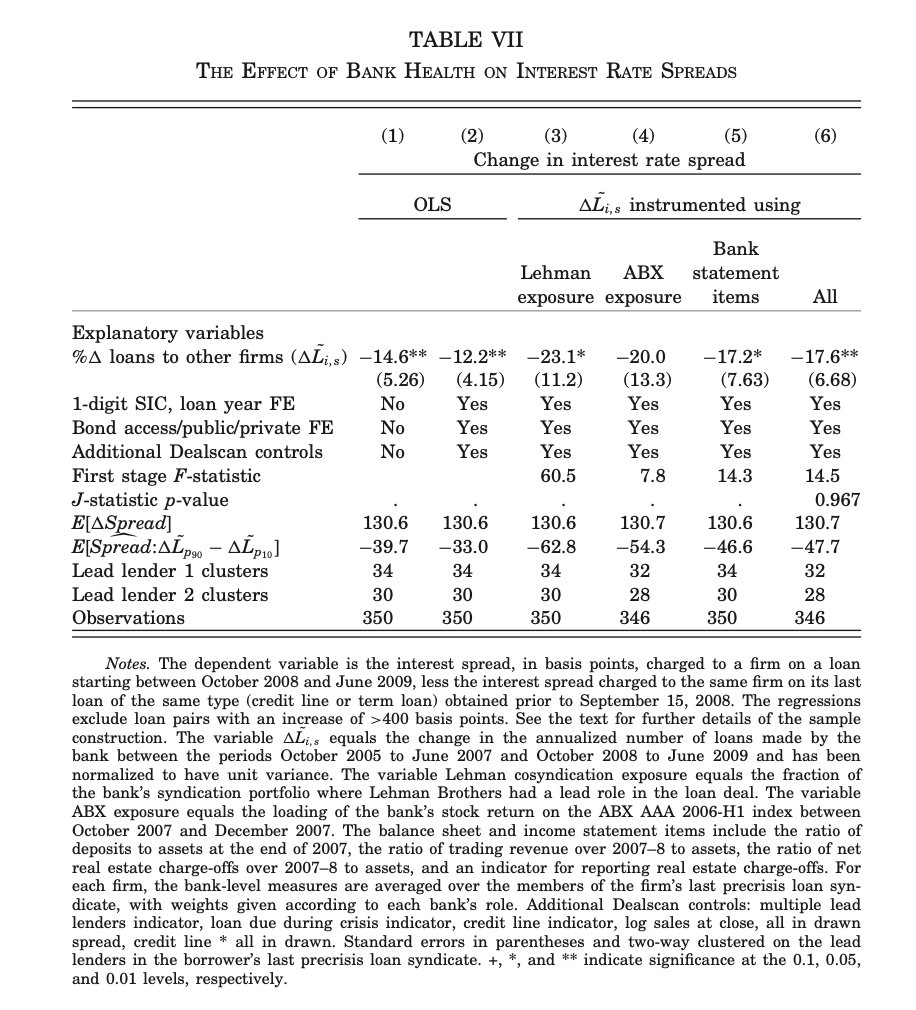
\includegraphics[scale=0.45]{figures/cr_3}
\end{figure}
\end{frame}


\begin{frame}{Results on Employment}
\begin{figure}
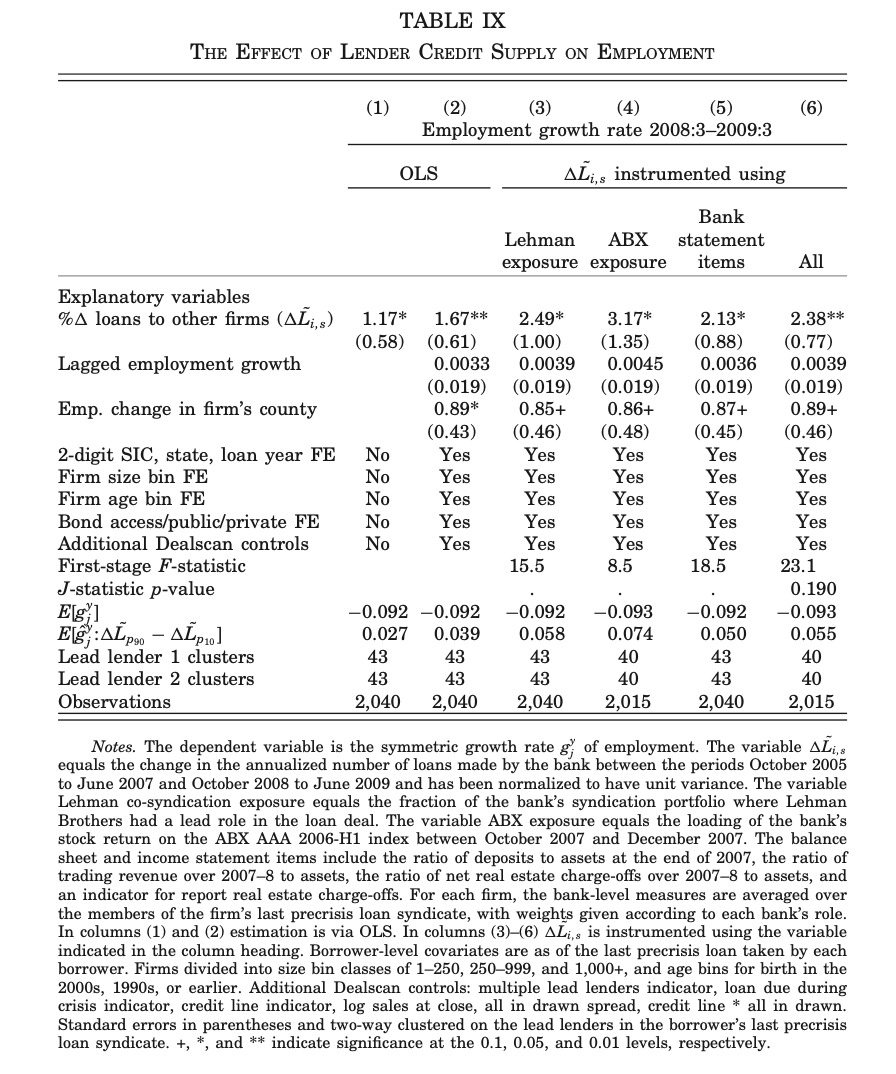
\includegraphics[scale=0.45]{figures/cr_4}
\end{figure}
\end{frame}

\begin{frame}{Counterfactual}

\end{frame}

\section{Huber 2018}


\begin{frame}{Huber 2018}
\begin{itemize}
\item The allies were convinced that the ability of Germany to wage war came from economic centralization
\item From 1948 to 1957, broke up three major banks and created banking zones
\item Firms form ties with banks close to them (Degryse and Ongena 2005)
\item Commerzbank had three HQ's
\item Instrument: Distance to a Commerzbank HQ
\end{itemize}
\end{frame}

\begin{frame}{Results}
\begin{figure}
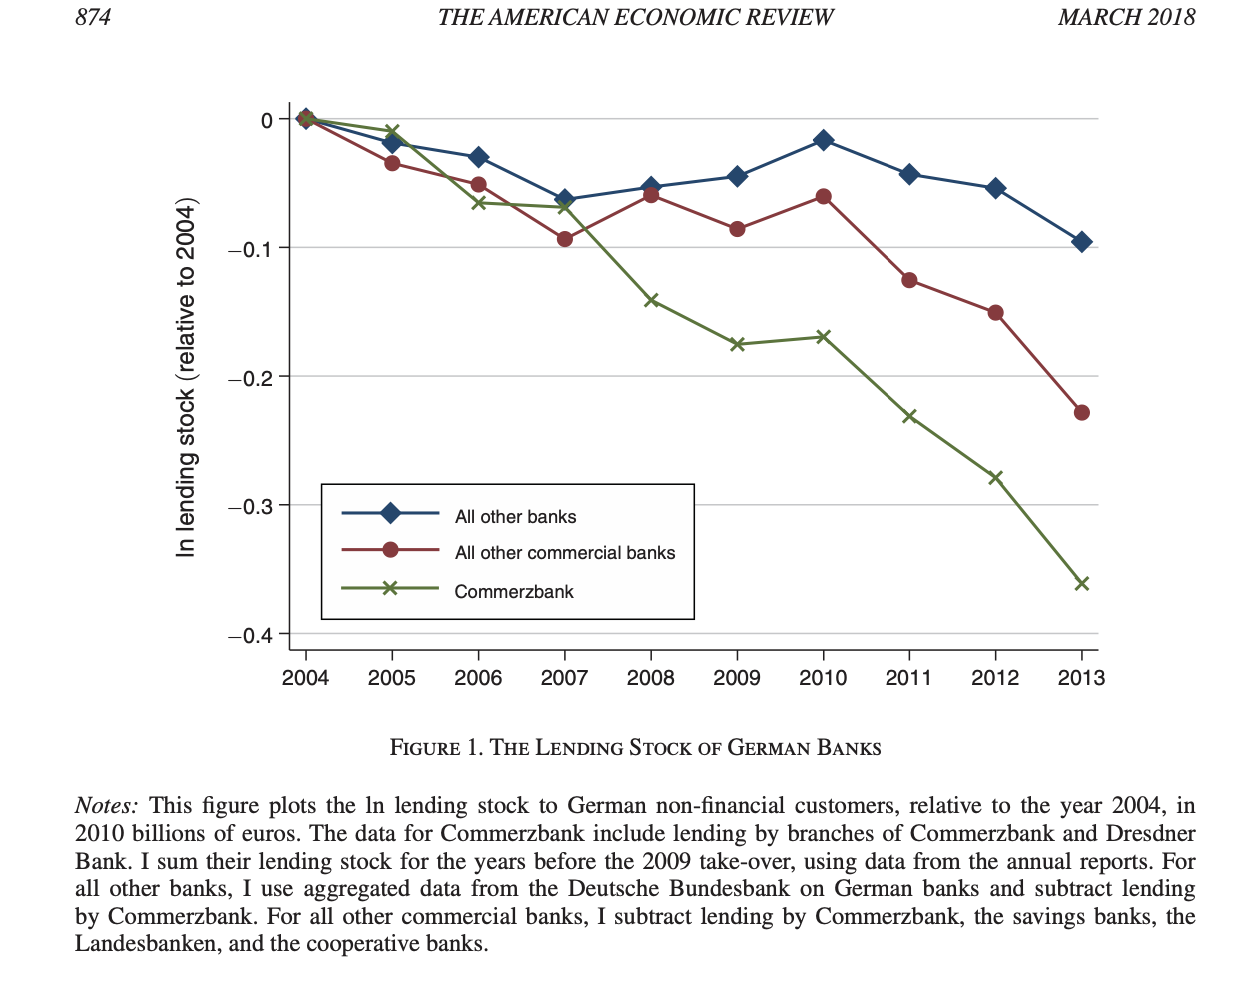
\includegraphics[scale=0.45]{figures/huber_1}
\end{figure}
\end{frame}


\begin{frame}{Specification}
\begin{itemize}
\item Firm-level effects
\[y_{fct} = \zeta  + \beta CBdep_{fc} \times d^{post}_t +\kappa_c\times d^{post}_t + \Gamma' X_{fc} \times d^{post}_t + \gamma_{cf} + \lambda_t + \epsilon_{fct} \]
\item Thoughts?
\end{itemize}
\end{frame}


\begin{frame}{Results}
\begin{figure}
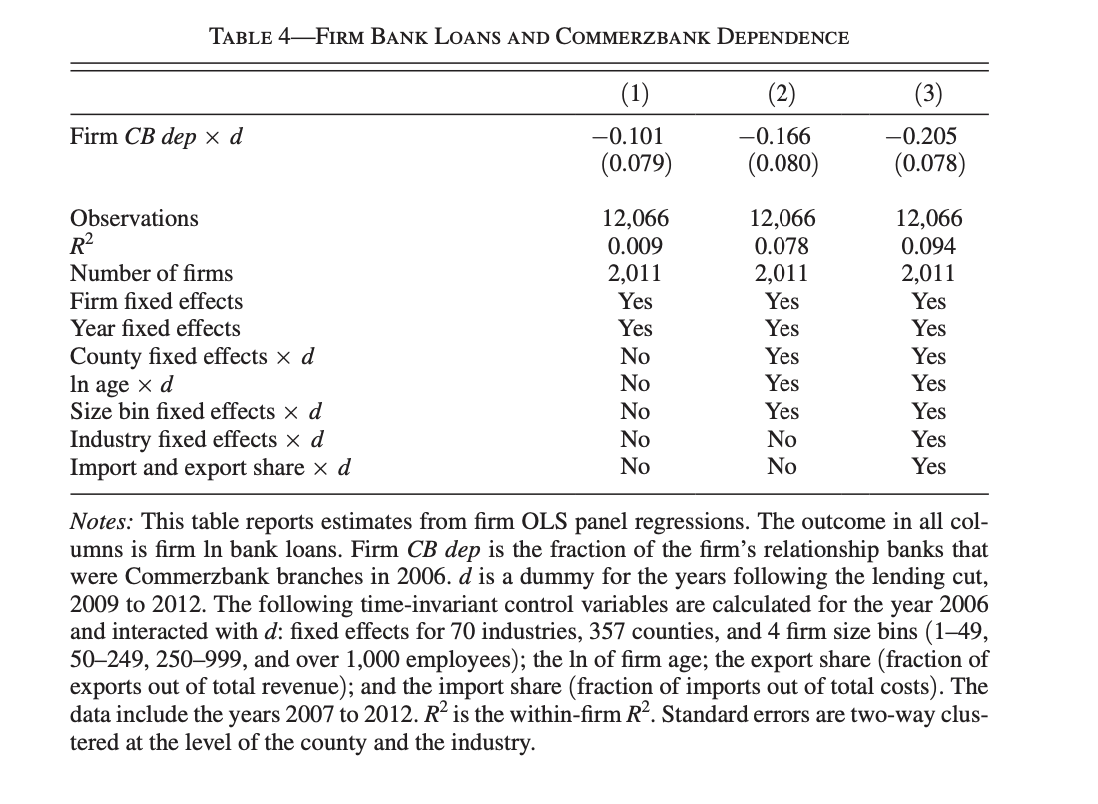
\includegraphics[scale=0.45]{figures/huber_2}
\end{figure}
\end{frame}

\begin{frame}{Results}
\begin{figure}
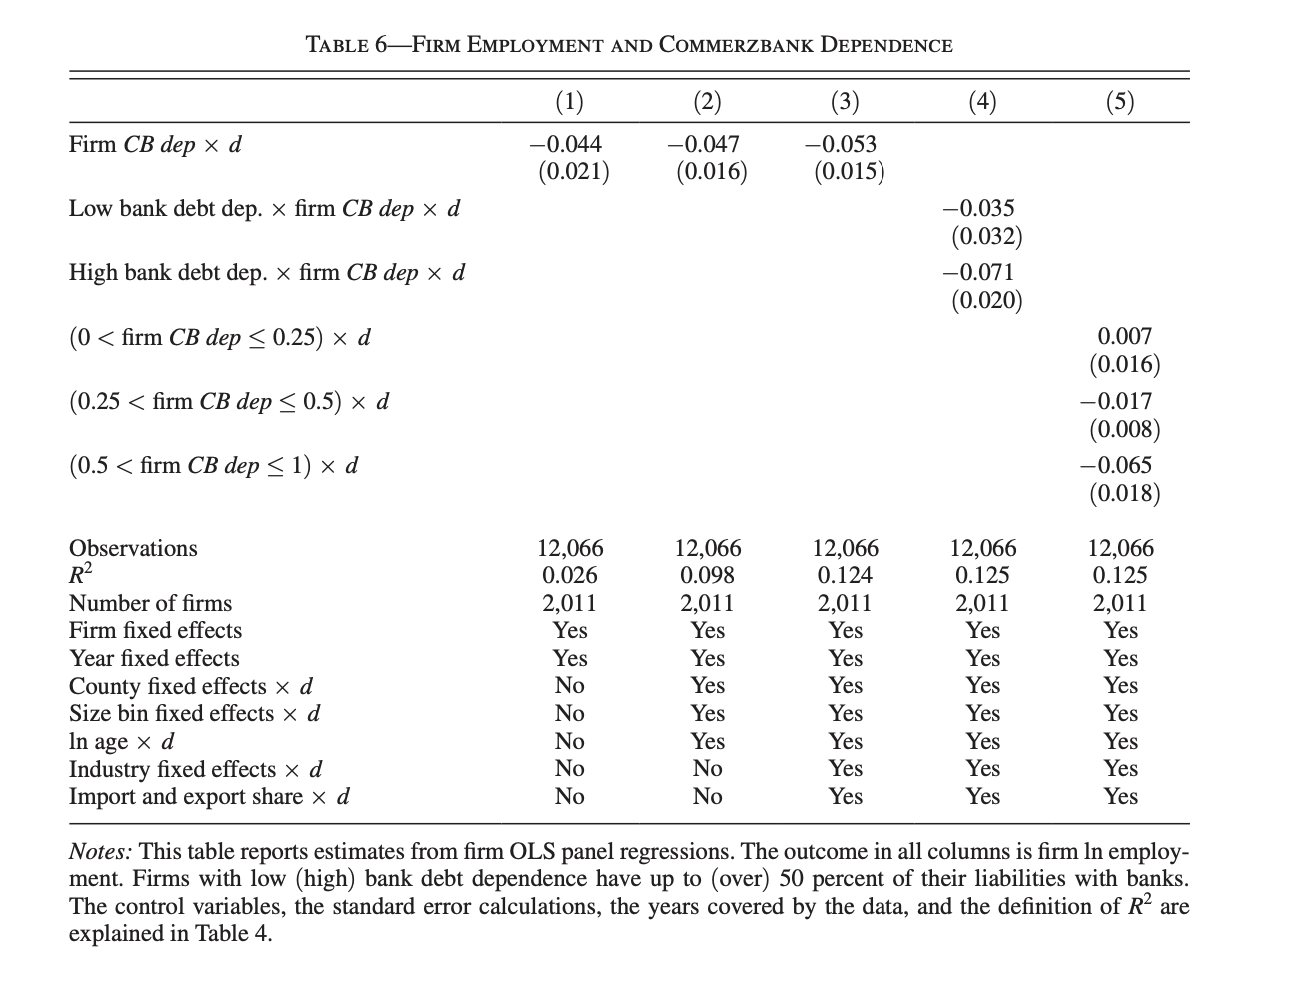
\includegraphics[scale=0.45]{figures/huber_3}
\end{figure}
\end{frame}


\begin{frame}{Results}
\begin{figure}
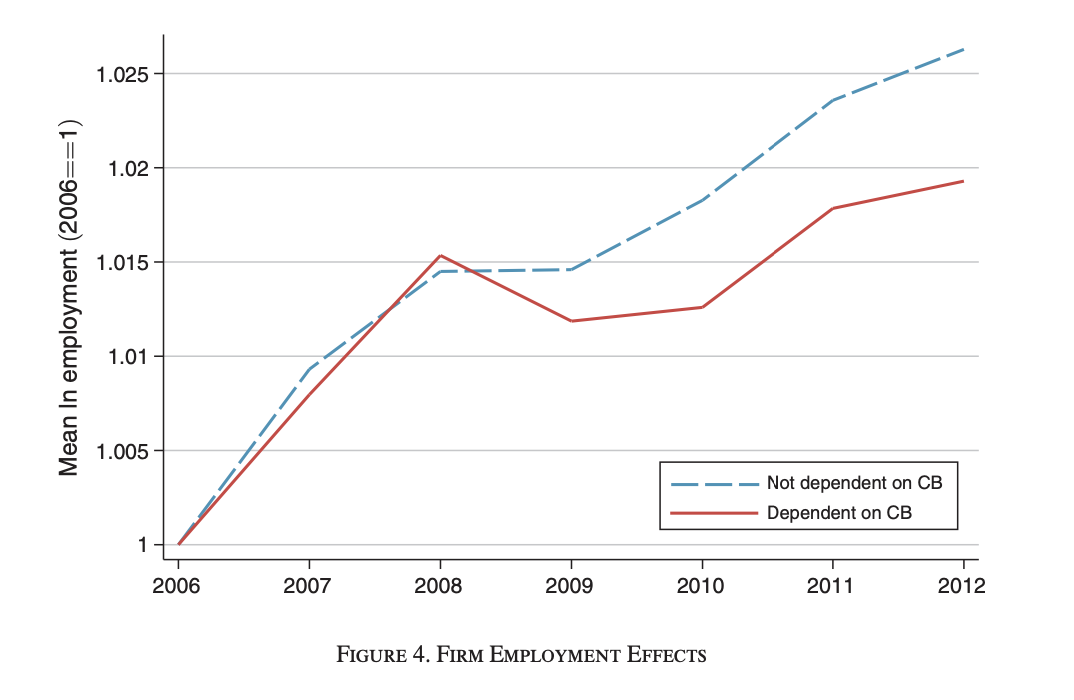
\includegraphics[scale=0.45]{figures/huber_4}
\end{figure}
\end{frame}

\begin{frame}{County Specification}
\begin{itemize}
\item Aggregate at the county level using average exposure
\[y_{ct} = \zeta + \rho \overline{CBdep_c} \times d^{post}_t + \Gamma' X_{c} \times d^{post}_t + \gamma_{c} + \lambda_t + \epsilon_{fct} \]
\end{itemize}
\end{frame}


\begin{frame}{Results}
\begin{figure}
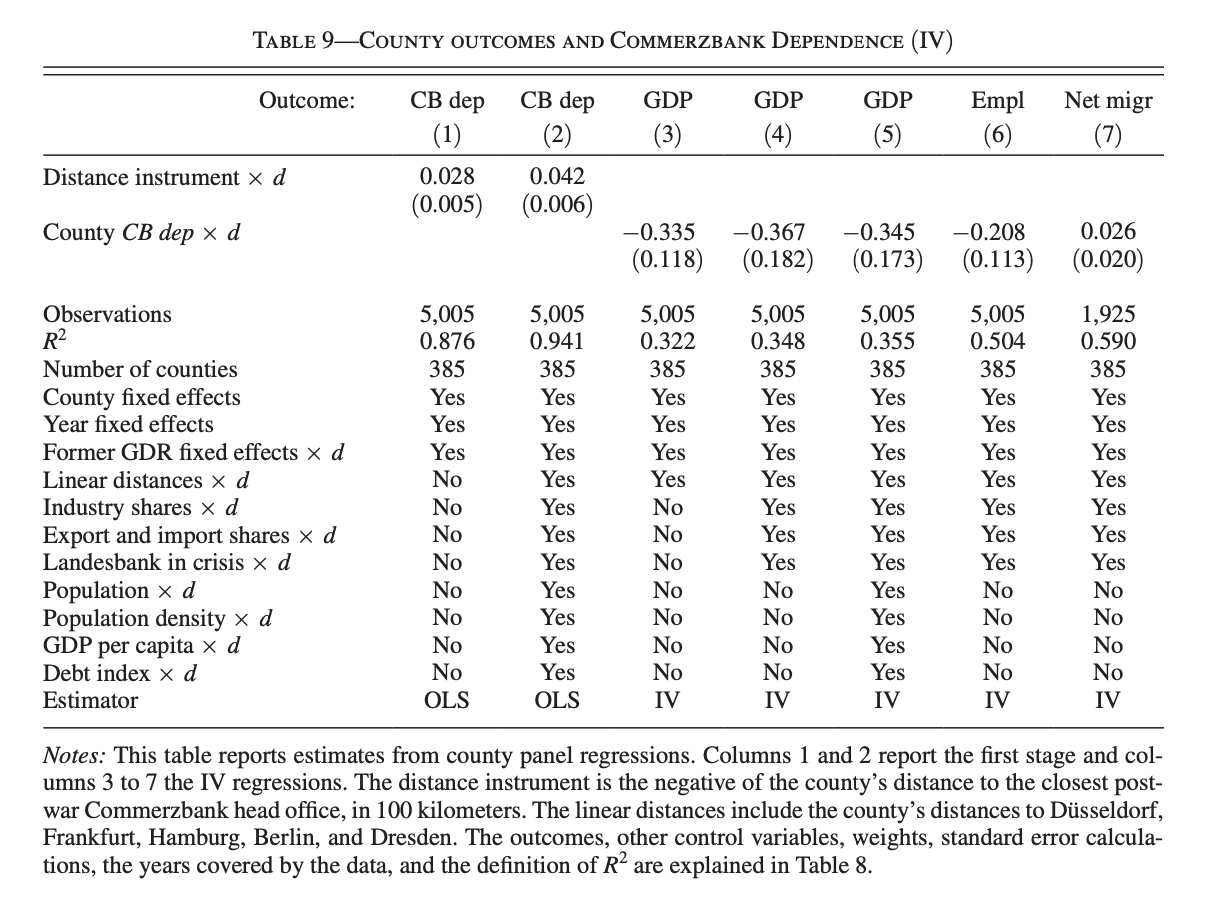
\includegraphics[scale=0.45]{figures/huber_5}
\end{figure}
\end{frame}

\begin{frame}{Indirect Effects}
\begin{itemize}
\item Estimate spillovers in local economies
\[\Delta y_{fc} = \zeta +  \beta {CBdep_{fc}} +  \sigma \overline{CBdep_{fc}}  + \Gamma' X_{fc} +  \xi{fc} \]
\end{itemize}
\end{frame}

\begin{frame}{Results}
\begin{figure}
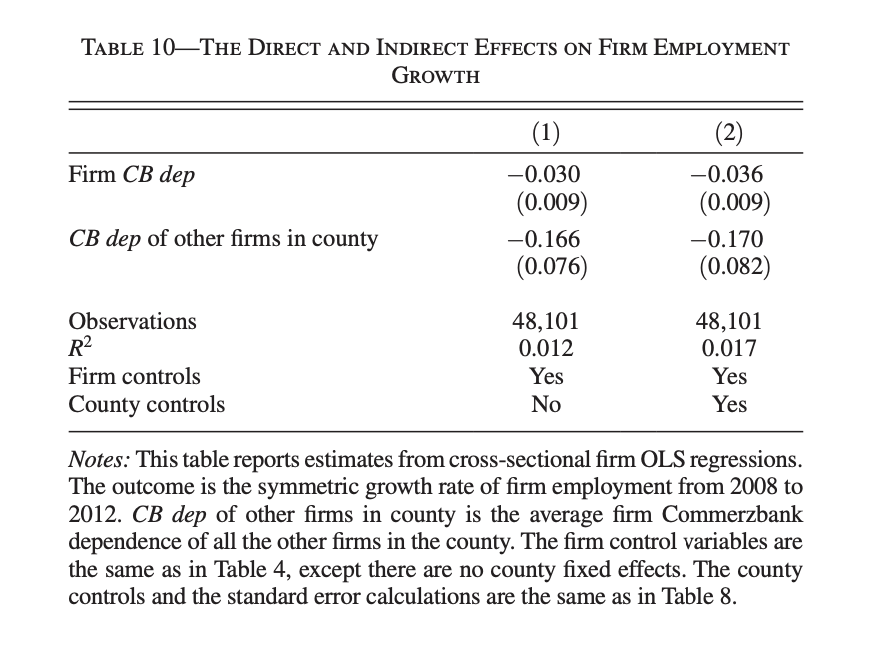
\includegraphics[scale=0.45]{figures/huber_6}
\end{figure}
\end{frame}

\begin{frame}{Question}
Regional effects in general are not equal to aggregate effects. In this setting what is the main concern to aggregation at the national level?
\end{frame}

\section{Herre\~no (2022)}


\begin{frame}{Production and Hiring}
\begin{itemize}
\item Produce by mixing a continuum of intermediates ($\omega$)
\begin{align*}
Y_{j} = \left(\int_{0}^{1} y_{j}(\omega)^{\frac{\sigma-1}{\sigma}} d\omega\right)^{\frac{\sigma}{\sigma - 1}}
\end{align*}
\item Each intermediate is produced with labor
$$y_{j}(\omega) = z_{j}  l_{j}(\omega)$$
\end{itemize}
\end{frame}

\begin{frame}{Cost minimization problem}\label{cm}

Total cost of producing $\omega$
$$TC_{j}(\omega) = \frac{w_j}{z_j} R_j(\omega)  y_j(\omega)$$


Minimize cost s.t. a target quantity $Y_j$
$$\min_{y_j(\omega)} \int_0^1 TC_{j}(\omega) d\omega \text{   ;   s.t.}  Y_{j} \geq \bar{Y} $$

Standard except for $R_j(\omega)$\\
\hyperlink{cm_details}{\beamerbutton{More Details}}
\end{frame}


\begin{frame}{Financing}
\begin{itemize}
\item $N_{\mathcal{B}}$ bank types, and 1 self-finance option
\item For each $\omega$ the firm picks the best option
\item $\epsilon$ are shifters that reflect the specificity of funding for a given task
$${R}_j(\omega) =  \min \left\lbrace\frac{R_{\mathcal{S}}}{\epsilon_{j\mathcal{S}}(\omega)}, \frac{R_{1}}{\epsilon_{j1}(\omega)}, ..., \frac{R_{N_{\mathcal{B}}}}{\epsilon_{jN_{\mathcal{B}}}(\omega)}\right\rbrace$$
\item Choose one (and only one) financing option for $\omega$
\end{itemize}
\end{frame}


\begin{frame}{Distribution of shifters}
The vector $\bm{\epsilon} = \{\epsilon_{j,1,\mathcal{B}}, ... , \epsilon_{j,N_{\mathcal{B}},\mathcal{B}},\epsilon_{j,N_{\mathcal{B}},\mathcal{B}},...  \epsilon_{j,N_{\mathcal{S}},\mathcal{S}} \}$ drawn from a nested Fr\'echet Distribution

$$F_j(\bm{\epsilon}) = \exp{\left\lbrace- \sum_{f \in (\mathcal{B},\mathcal{S})} \bar{\varphi}_f \left( \sum_{b = 1}^{N_{f}}  T_{jb} \epsilon_{fb}^{-\theta} \right)^{\frac{\varphi}{\theta}} \right\rbrace}$$
\begin{itemize}
\item $\theta$ dictates dispersion of shifters across banks
\item $\varphi$ dictates dispersion of shifters across financing type
\end{itemize}
\end{frame}
%
%\begin{frame}{Analytical results}
%The share of intermediates financed with bank $b$ is given by $ \nu_{jb} s_j$
%\begin{enumerate}
%\item $s_j$: The expenditures share financed with the banking sector
%\item $\nu_{jb}$: The share of bank credit from bank $b$
%\end{enumerate}
%\end{frame}



\begin{frame}{Allocation of bank borrowing}
Firm $j$ borrows from bank $b$ a fraction $\nu_{jb}$ of its bank-credit needs
\begin{minipage}[t]{0.48\linewidth}
\begin{align*}
\nu_{jb} = \frac{T_{jb} R_{b}^{-{\color{red}{\theta}}}}{\sum_{k = 1}^{N_{\mathcal{B}}} T_{jk} R_{k}^{-{\color{red}{\theta}}}}
\end{align*}
\begin{align*}
R_{jB} = \left(\sum_{k = 1}^{N_{\mathcal{B}}} T_{jk} R_{k}^{-\theta}\right)^{-1/\theta}
\end{align*}
\end{minipage}\hfill
\begin{minipage}[t]{0.48\linewidth}
\vspace{0pt}
\begin{figure}
\centering
\begin{tikzpicture}[scale=0.7]
\draw [thick] (0,0) node [below] {} -- (0,0) -- (5.5,0) node [below] {$\nu_{jb}$};
\draw [thick] (0,0) node [below] {} -- (0,0) -- (0,5.5) node [left] {$R_{b}$};
\draw [thick,color=red] (1.3,5.5) to [bend right=30] (5.5,0.5) node [right] {$\theta_{low}$};
\draw [thick,dashdotted,color=orange] (0,2.45) to (5.5,2.45) node [right] {$\theta_{\infty}$};
\draw [thick,dashdotted,color=cyan] (2.6,0) to (2.6,5.5) node [right] {$\theta_{0}$};
\draw  [thick, color=blue] plot [smooth] coordinates {(0,4) (3.3,2.1) (5.5,1.5)} node [right] {$\theta_{high}$};
\end{tikzpicture}
\end{figure}
\end{minipage}
\\
${\color{red}{\theta}}$ is the elasticity of substitution across bank types
\end{frame}

%
%\begin{frame}{Allocation of bank borrowing}
%Fraction of bank credit coming from bank $b$
%$$\nu_{jb} = \frac{T_{jb}R_{b}^{-\theta}}{\sum_{k = 1}^{N_{\mathcal{B}}} T_{jk}R_{k}^{-\theta}}$$
%Faces a bank-credit cost of funds $R_{jB}$
%\begin{align*}
%R_{jB} = \left(\sum_{k = 1}^{N_{\mathcal{B}}} T_{jk} R_{k}^{-\theta}\right)^{-1/\theta}
%\end{align*}
%
%\end{frame}


\begin{frame}{Credit Dependence}
Firm $j$ finances a fraction $s_{j}$ of its working capital
\begin{minipage}[t]{0.48\linewidth}
\begin{align*}\label{eq:financing_share}
s_{j} = \frac{\bar{\varphi} R_{jB}^{-{\color{red}{\varphi}}}}{\bar{\varphi} R_{jB}^{-{\color{red}{\varphi}}} +(1-\bar{\varphi})R_{jS}^{-{\color{red}{\varphi}}} }
\end{align*}
\begin{align*}
R_{j} = \left(\bar{\varphi} R_{jB}^{-\varphi} + (1-\bar{\varphi})  R_{jS}^{-\varphi}\right)^{-1/\varphi}
\end{align*}
\end{minipage}\hfill
\begin{minipage}[t]{0.45\linewidth}
\begin{figure}
\centering
\begin{tikzpicture}[scale=0.7]
\draw [thick] (0,0) node [below] {} -- (0,0) -- (5.5,0) node [below] {$s_{j}$};
\draw [thick] (0,0) node [below] {} -- (0,0) -- (0,5.5) node [left] {$R_{jB}$};
\draw [thick,color=red] (1.3,5.5) to [bend right=30] (5.5,0.5) node [right] {$\varphi_{low}$};
\draw [thick,dashdotted,color=orange] (0,2.45) to (5.5,2.45) node [right] {$\varphi_{\infty}$};
\draw [thick,dashdotted,color=cyan] (2.6,0) to (2.6,5.5) node [right] {$\varphi_{0}$};
\draw  [thick, color=blue] plot [smooth] coordinates {(0,4) (3.3,2.1) (5.5,1.5)} node [right] {$\varphi_{high}$};
\end{tikzpicture}
\end{figure}
\end{minipage}\\
${\color{red}{\varphi}}$ is the elasticity of substitution of bank-credit
\end{frame}

%
%\begin{frame}{Share of bank borrowing}
%Firm $j$ borrows a fraction of its expenditures $s_{j}$ with banks
%$$s_{j} = \frac{\bar{\varphi} R_{jB}^{-\varphi}}{\bar{\varphi} R_{jB}^{-\varphi} + (1-\bar{\varphi})  R_{jS}^{-\varphi}}$$
%Faces a bank-credit cost of funds $R_{jBt}$
%\begin{align*}
%R_{j} = \left(\bar{\varphi} R_{jB}^{-\varphi} + (1-\bar{\varphi})  R_{jS}^{-\varphi}\right)^{-1/\varphi}
%\end{align*}
%\end{frame}


\begin{frame}{Households}
Representative household maximizes utility
$$U(C,L) = \frac{1}{1-\gamma} \left(C   - \frac{L^{\xi + 1}}{\xi  + 1}\right)^{1-\gamma}$$
$C$ is a Dixit-Stiglitz aggregator
\begin{align*}
C = \left(\int_0^1 C_{j}^{\frac{\eta-1}{\eta}} dj\right)^{\frac{\eta}{\eta-1}} 
\end{align*}
$L$ is an aggregator of the labor supplied to different firms
\begin{align*}
L = \left(\int_0^1 L_{j}^{\frac{1+\alpha}{\alpha}} dj\right)^{\frac{\alpha}{1+\alpha}} 
\end{align*}
Subject to
$$C_t = \int_0^1 w_j L_j  dj + \int_0^1 \Pi_{j} dj$$
\end{frame}
%
%\begin{frame}{Firm Problem - Revisited}
%Firm maximize profits
%$$\Pi_j = P_j Y_j  - w_j L_j R_j$$
%
%Subject to:
%$$R_{j} = \left(\bar{\varphi} R_{jB}^{-\varphi} + (1-\bar{\varphi})  R_{jS}^{-\varphi}\right)^{-1/\varphi}$$
%
%$$R_{jB} = \left(\sum_{k = 1}^{N_{\mathcal{B}}} T_{jk} R_{k}^{-\theta}\right)^{-1/\theta}$$
%
%$$Y_j = Y P_j^{-\eta}$$
%\end{frame}



\begin{frame}{Experiment 1: Funding shock to all the banks}
\begin{itemize}
\item Increase banks funding cost from $R$ to $Re^u$ for small u
\item Keep the self-financing rate at $R$
\end{itemize}
Characterize aggregate output drop up to the second order
\end{frame}


\begin{frame}{Aggregate effects of an across-the-board bank disruption}
$$\log Y - \log \bar{Y} \approx - \frac{1}{{\color{red}{\xi}}}  \bar{s}  \left(u - {\color{red}{\varphi}} (1-\bar{s}) \frac{u^2}{2} - \Omega \frac{u^2}{2}\right)$$
Large aggregate response under
\begin{enumerate}
\item Elastic labor supply  ($1/\xi$ large)
\item Low substitutability of bank credit ($\varphi$ small)
\end{enumerate}
\end{frame}


\begin{frame}{Experiment 2: increase the lending rate of one bank}
\begin{itemize}
\item Increase the funding rate of bank $b$ from $R$ to $Re^u$ for small $u$
\item Keep the funding costs of every other bank at $R$
\item Keep self finance rate $R_S = R$
\end{itemize}
Characterize fall in aggregate output up to a second order
\end{frame}

\begin{frame}{Aggregate effects of a one-bank disruption}\label{agg_1_2nd}
\begin{align*}
\log Y - \log \bar{Y} \approx  -\frac{1}{{\color{red}{\xi}}} \bar{s} \left(\nu_b u - {\color{red}{\theta}}\frac{u^2}{2}\Upsilon_1- {\color{red}{\varphi}}(1-\bar{s}) \frac{u^2}{2}\Upsilon_2  - \Omega \Upsilon_2 \frac{u^2}{2}\right)
\end{align*}
Larger effects when
\begin{enumerate}
\item Elastic labor supply  ($1/\xi$ large)
\item Firms do not substitute across banks ($\theta$ small)
\item Firms do not switch away from bank credit ($\varphi$ small)
\end{enumerate}
\end{frame}


%
%
%
\begin{frame}{Cross-Sectional effects on ouput}
$$\Delta \log \text{Output}_{j} = \beta_0 + \beta_{\text{output}} T_{jb} + \epsilon_{j}$$
%\begin{minipage}[t]{0.48\linewidth}
%\vspace{0pt}
%\end{minipage}\hfill
%\begin{minipage}[t]{0.48\linewidth}
%\vspace{0pt}
\begin{figure}[H]
\centering
\begin{tikzpicture}[scale=0.7]
\draw [thick] (0,0) node [below] {} -- (0,0) -- (5.5,0) node [below] {$\varphi$};

\draw [thick] (0,0) node [below] {} -- (0,0) -- (0,5.5) node [left] {$\theta$};
\node at (1,4.45)[circle,fill,inner sep=1.5pt]{};
\draw [dashed] (1,0) node [below] {$\varphi_1$} (1,0) -- (1,4.45);
\draw [dashed] (0,4.45) node [left] {$\theta_1$} (0,4.45) -- (1,4.45);
\draw [dashed] (3.3,0) node [below] {$\varphi_2$} ;
\node at (3.3,3.1)[circle,fill,inner sep=1.5pt]{};
\draw [dashed] (3.3,0) -- (3.3,3.1);
\draw [dashed] (0,3.1) node [left] {$\theta_2$} (0,3.1) -- (3.3,3.1);
\draw plot [smooth] coordinates {(0.5,4.8) (1,4.45) (2,3.95) (3.3,3.1) (4,2.5) (5,1.5)};
\node [right] at (5,1.5) {$\beta_{output}$};
\end{tikzpicture}
\end{figure}
%\end{minipage}
$$\beta_{\text{output}} \approx -  \frac{\eta \alpha}{\alpha+\eta} \bar{s} u\left(1 - \theta  \frac{u}{2}\mathcal{M}_1 - \varphi (1-\bar{s}) \frac{u}{2} \mathcal{M}_2\right)$$
\end{frame}



\begin{frame}{Cross-Sectional effects on credit}
$$\Delta \log \text{Loans}_{j} = \beta_0 + \beta_{\text{loans}} T_{jb} + \epsilon_{j}$$
%\begin{minipage}[t]{0.48\linewidth}
%\vspace{0pt}
%\end{minipage}\hfill
%\begin{minipage}[t]{0.48\linewidth}
%\vspace{0pt}
\begin{figure}[H]
\centering
\begin{tikzpicture}[scale=0.7]
\draw [thick] (0,0) node [below] {} -- (0,0) -- (5.5,0) node [below] {$\varphi$};

\draw [thick] (0,0) node [below] {} -- (0,0) -- (0,5.5) node [left] {$\theta$};
\node at (2,2.4)[circle,fill,inner sep=1.5pt]{};
\draw [dashed] (2,0) node [below] {$\varphi_1$} (2,0) -- (2,2.4);
\draw [dashed] (0,2.4) node [left] {$\theta_1$} (0,2.4) -- (2,2.4);
\draw [dashed] (4,0) node [below] {$\varphi_2$} ;
\node at (4,3.6)[circle,fill,inner sep=1.5pt]{};
\draw [dashed] (4,0) -- (4,3.6);
\draw [dashed] (0,3.6) node [left] {$\theta_2$} (0,3.6) -- (4,3.6);
\draw plot [smooth] coordinates {(0.5,2) (1,2.1) (2,2.4) (3.3,3.1) (4,3.6) (5,4.7)};

\node [right] at (5,4.7) {$\beta_{\text{loans}}$};
\end{tikzpicture}
\end{figure}
%\end{minipage}
$$\beta_{\text{credit}} \approx \beta_{\text{output}}\frac{\alpha+1}{\alpha} - \varphi(1-s)u\left(1+ \varphi \frac{u}{2}s \mathcal{M}_1 - \theta \frac{u}{2} \mathcal{M}_2\right)$$
\end{frame}


\begin{frame}{Identification}\label{identification_theory}
%\begin{minipage}[t]{0.48\linewidth}
%\vspace{0pt}
%\end{minipage}\hfill
%\begin{minipage}[t]{0.48\linewidth}
%\vspace{0pt}
\begin{figure}[H]
\centering
\begin{tikzpicture}[scale=0.7]
\draw [thick] (0,0) node [below] {} -- (0,0) -- (5.5,0) node [below] {$\varphi$};
\draw [thick] (0,0) node [below] {} -- (0,0) -- (0,5.5) node [left] {$\theta$};
\draw plot [smooth] coordinates {(0.5,4.8) (1,4.45) (2,3.95) (3.3,3.1) (4,2.5) (5,1.5)};
\node [right] at (5,1.5) {$\beta_{\text{output}}$};
\draw plot [smooth] coordinates {(0.5,2) (1,2.1) (2,2.4) (3.3,3.1) (4,3.6) (5,4.7)};
\node [right] at (5,4.7) {$\beta_{\text{loans}}$};
\node at (3.3,3.1)[circle,fill,inner sep=1.5pt]{};
\end{tikzpicture}
\end{figure}
%\end{minipage}
Recover $\theta$ and $\varphi$ conditional on knowing $\alpha, \eta$
\\
\hyperlink{locus_numerical}{\beamerbutton{Back}}
\end{frame}

%\begin{frame}{Effect of labor market frictions}
%\begin{minipage}[t]{0.48\linewidth}
%Higher $\alpha$ displaces both loci
%\begin{figure}[H]
%\centering
%\begin{tikzpicture}[scale=0.7]
%\draw [thick] (0,0) node [below] {} -- (0,0) -- (5.5,0) node [below] {$\varphi$};
%\draw [thick] (0,0) node [below] {} -- (0,0) -- (0,5.5) node [left] {$\theta$};
%\draw [thick,dashdotted,color=gray] plot [smooth] coordinates {(0.5,4.8) (1,4.45) (2,3.95) (3.3,3.1) (4,2.5) (5,1.5)};
%\node [right] at (5,1.5) {$\beta_{\text{output}}$};
%\draw [thick,dashdotted,color=gray]  plot [smooth] coordinates {(0.5,2) (1,2.1) (2,2.4) (3.3,3.1) (4,3.6) (5,4.7)};
%\node [right] at (5,4.7) {$\beta_{\text{loans}}$};
%\pause
%\draw [thick,color=gray] plot [smooth] coordinates {(2,5.5) (2.5,5.25) (3.5,4.55) (4.8,3.8) (5.6,3.2) (6.5,2.5)} ;
%\node [right] at (6.5,2.5) {$\beta_{\text{output}}$};
%\pause
%\draw [thick,color=gray]  plot [smooth] coordinates {(0.2,2.3) (0.7,2.4) (1.7,2.7) (3,3.5) (3.7,3.9) (4.7,5)};
%\node [above] at (4.7,5) {$\beta_{\text{loans}}$};
%\pause
%\node at (3.3,3.1)[circle,fill,inner sep=1.5pt]{};
%\node at (4.04,4.21)[circle,fill,inner sep=1.5pt]{};
%\end{tikzpicture}
%\end{figure}
%\end{minipage}%
%\begin{minipage}[t]{0.48\linewidth}
%With a higher $\alpha$
%\begin{itemize}
%\item $\beta_{\text{output}}$: Higher $\varphi$ and $\theta$
%\item $\beta_{\text{loans}}$: Higher $\theta$ and lower $\varphi$
%\end{itemize}
%\end{minipage}
%%\end{minipage}
%\end{frame}

\begin{frame}{Firm fixed-effect regressions}
$$\Delta \log \text{Loans}_{jb} = \beta_j + \beta_{\text{fe}} T_{jb} + \epsilon_{jb}$$
In the model, the fixed-effect elasticity
\begin{align}
\beta_{\text{fixed effect}} \approx - \theta u + \theta^2 \frac{u^2}{2} \mathcal{M}_1
\end{align}
Contains no information about $\varphi$
\end{frame}


\begin{frame}{Observational equivalence}
$$\Delta \log \text{Output}_{j} = \beta_0 + \beta_{\text{output}} T_{jb} + \epsilon_{j}$$

$$\beta_{\text{output}} \approx -  \frac{\eta \alpha}{\alpha+\eta} \bar{s} u\left(1 - \theta  \frac{u}{2}\mathcal{M}_1 - \varphi (1-\bar{s}) \frac{u}{2} \mathcal{M}_2\right)$$
Alternative worlds consistent with small elasticities
\begin{enumerate}
\item Firms are elastic in subsituting sources of finance ($\varphi$, $\theta$ large)
\item Firm-specific labor supply is inelastic ($\alpha$ small)
\item Varieties are not substitutable ($\eta$ small)
\end{enumerate}
Different assumptions of $\alpha$, $\eta$, change inferred $\varphi, \theta$
\end{frame}


\begin{frame}{Observational equivalence}
$$\Delta \log \text{Output}_{j} = \beta_0 + \beta_{\text{output}} T_{jb} + \epsilon_{j}$$
%\begin{minipage}[t]{0.48\linewidth}
%\vspace{0pt}
%\end{minipage}\hfill
%\begin{minipage}[t]{0.48\linewidth}
%\vspace{0pt}
\begin{figure}[H]
\centering
\begin{tikzpicture}[scale=0.7]
\draw [thick] (0,0) node [below] {} -- (0,0) -- (5.5,0) node [below] {$\varphi$};

\draw [thick] (0,0) node [below] {} -- (0,0) -- (0,5.5) node [left] {$\theta$};
\draw plot [smooth] coordinates {(0.5,4.8) (1,4.45) (2,3.95) (3.3,3.1) (4,2.5) (5,1.5)};
\node [below] at (5,1.5) {};
\pause
\draw plot [smooth] coordinates {(2.5,4.8) (3,4.45) (4,3.95) (5.3,3.1) (6,2.5) (7,1.5)};
\node [right] at (7,1.5) {$\beta_{output}$};
\draw [->] (3.5,3.1) --  (5.1,3.1) node [left] {};

\end{tikzpicture}
\end{figure}
%\end{minipage}
$$\beta_{\text{output}} \approx -  \frac{\eta \alpha}{\alpha+\eta} \bar{s} u\left(1 - \theta  \frac{u}{2}\mathcal{M}_1 - \varphi (1-\bar{s}) \frac{u}{2} \mathcal{M}_2\right)$$
\end{frame}



\begin{frame}{Outline of the full model}\label{full_model}
Banks:
\begin{itemize}
\item Pay deposit rates to savers 
\item Maximize profits by setting lending rates \hyperlink{rate_setting}{\beamerbutton{Go there}}
\item Suffer balance sheet shocks: Equity drops
\end{itemize}
Firm owners
\begin{itemize}
\item Heterogeneous in wealth and productivity\hyperlink{het_entrep}{\beamerbutton{Go there}}
\item Own one particular firm
\item Deposit assets in banks  \hyperlink{deposits}{\beamerbutton{Go there}}
\end{itemize}
In continuous time to solve faster
\end{frame}



\begin{frame}{Allocation of deposits}\label{deposits}
Each entrepreneur allocates a share $\omega_{bt}$ of bank deposits to bank $b$
$$\omega_{bt} = \frac{R_{bd}^{\chi}}{\sum_{\forall k} {R_{kd}}^{\chi}}$$
\begin{itemize}
\item When $\chi \rightarrow \infty$ then savings are perfectly elastic
\item Analogous to the discrete choice block for lending
\item Very important. More competition in the banking sector $\chi$ large creates macro amplification
\end{itemize}

\end{frame}

\begin{frame}{Banks' balance sheets}\label{bank_bs}
\begin{align}
\text{Loans}_{bt} = \text{Deposits}_{bt} + \text{Equity}_{bt}
\end{align}

Total loans sum up loans to individual firms
\begin{align}
\text{Loans}_{bt} = \int_0^1 \text{Loans}_{jbt} dj  = \int_0^1 \text{Expenditure}_{jt} s_{jt}  \nu_{bjt} dj
\end{align}

Deposits sum up the deposits that banks get from every entrepreneur 

\begin{align}
\text{Deposits}_{bt} = \int_0^1 \text{Deposits}_{jbt} dj 
\end{align}
\hyperlink{exo_process}{\beamerbutton{Exogenous Driver}}
\hyperlink{sol_meth}{\beamerbutton{Solution Method}}
\end{frame}



\begin{frame}{Identification argument holds}\label{locus_numerical}
\begin{minipage}{0.4\textwidth}
\begin{figure}
\centering
\caption*{Elasticity of Credit}
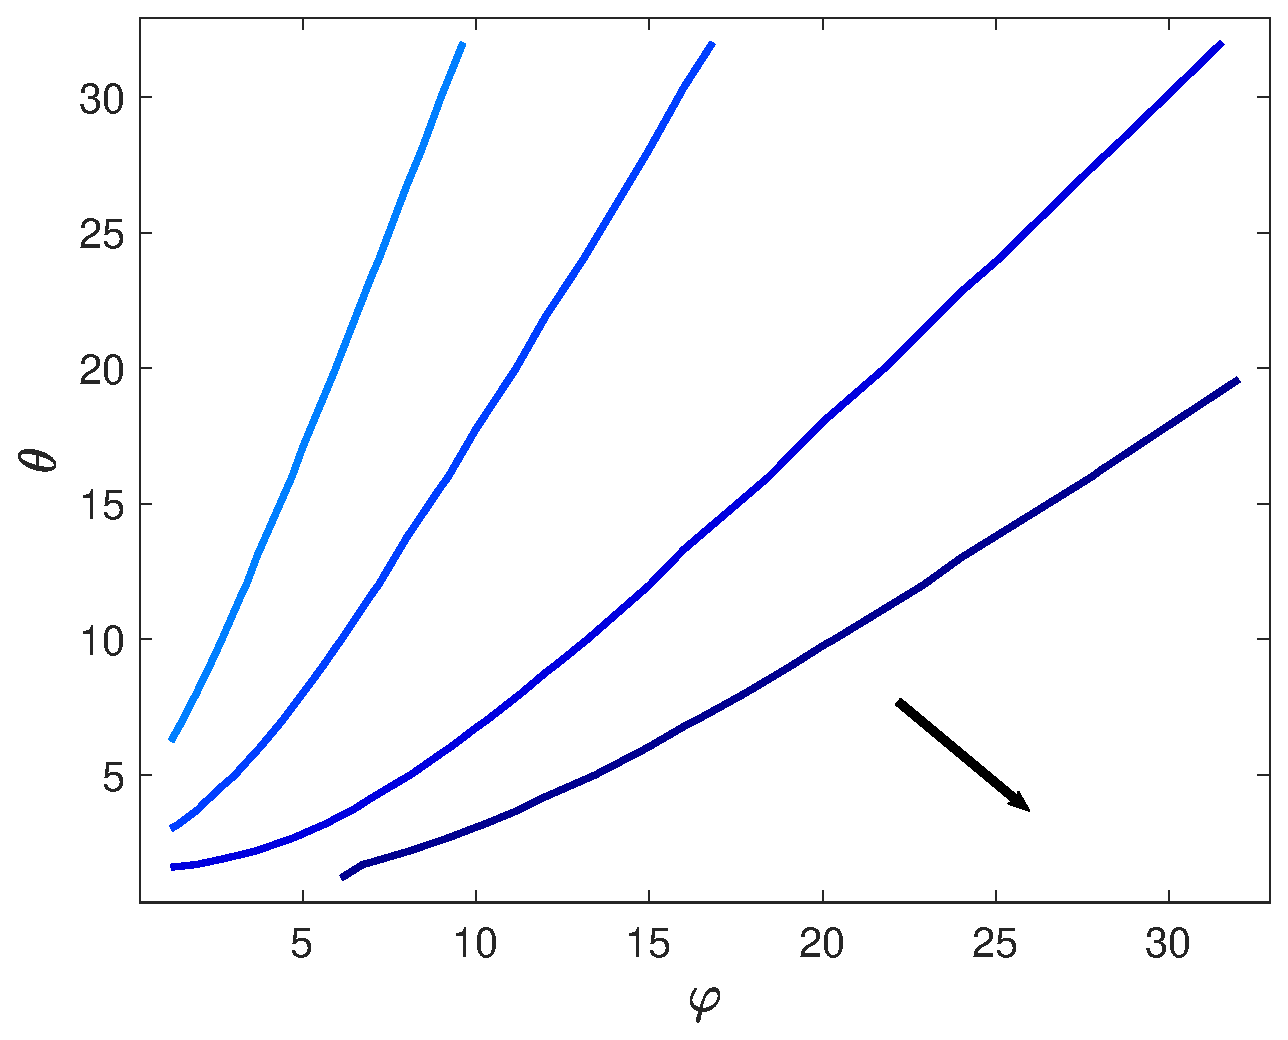
\includegraphics[scale=0.24]{Figures/huber_credit_varphi_theta_contour.eps}
\end{figure}
\end{minipage}\qquad
\begin{minipage}{0.4\textwidth}
\begin{figure}
\centering
\caption*{Elasticity of Employment}
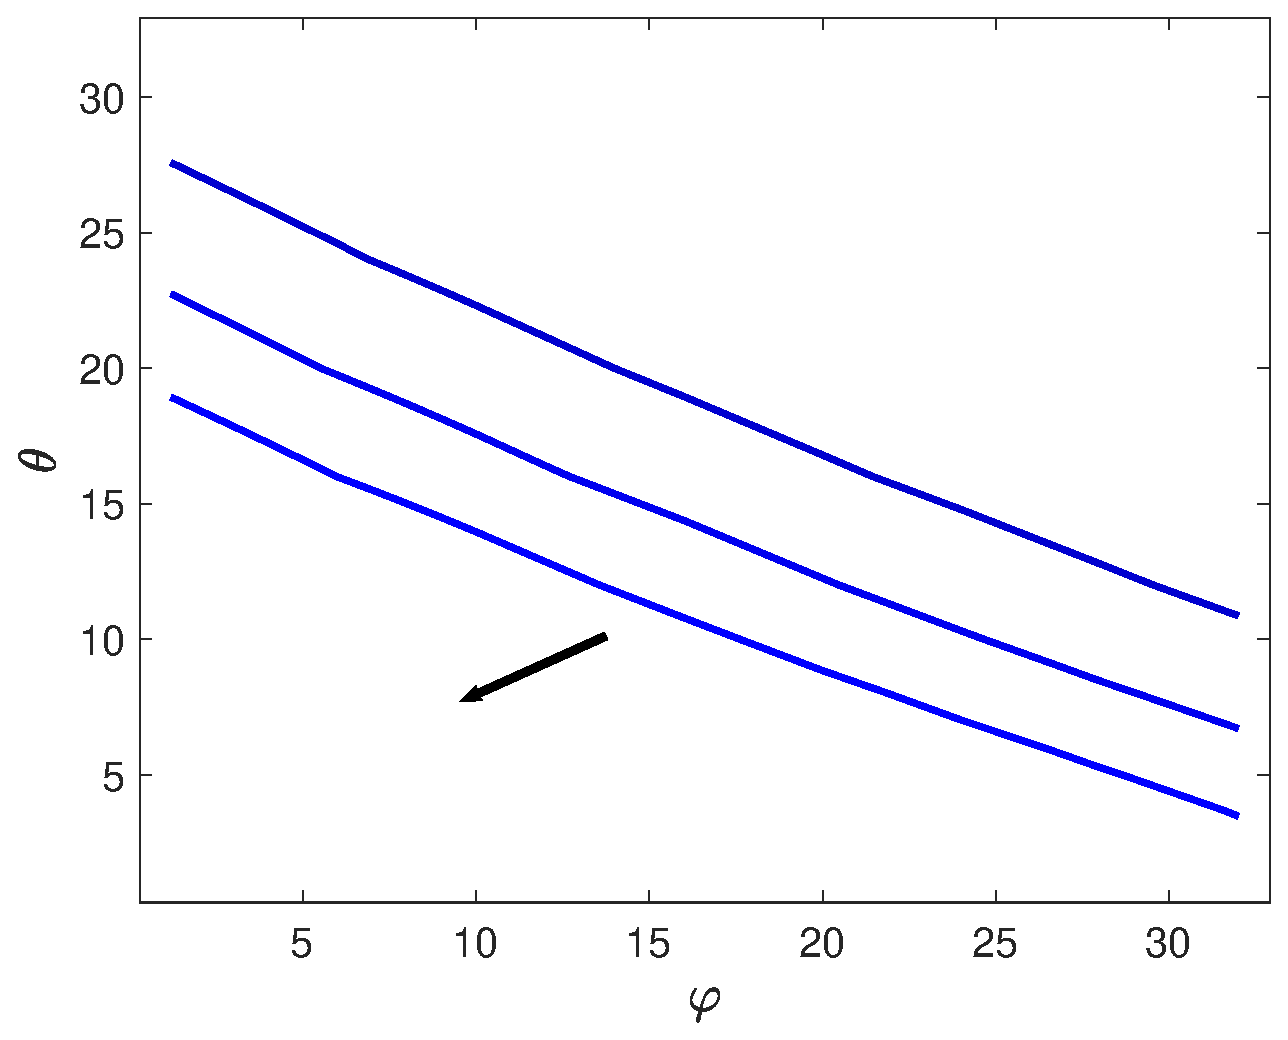
\includegraphics[scale=0.24]{Figures/huber_varphi_theta_contour.eps}
\end{figure}
\end{minipage}\\
\begin{enumerate}
\item Upward sloping locus for credit
\item Downward sloping locus for employment
\end{enumerate}
\hyperlink{identification_theory}{\beamerbutton{In the simple model}}
\hyperlink{locus_colors}{\beamerbutton{Sensitivities}}
\end{frame}



 
\begin{frame}{Aggregate Bank Shocks}
\begin{itemize}
\item Shock all the banks' equity at the same time
\end{itemize}
\end{frame}

\begin{frame}{Aggregate elasticity of output to lending}
We start by focusing on the elasticity of output to lending
\begin{align}
\varepsilon^M = \frac{\int_0^{\infty} e^{-\rho t} \left(\log(Y_t) - \log(\bar{Y})\right) dt} {\int_0^{\infty} e^{-\rho t} \left( \log(\text{Lending}_t)  - \log(\bar{\text{Lending}})\right) dt}
\end{align}

\begin{itemize}
\item The macroeconomic equivalent of an IV estimate. Ratio of:
\begin{itemize}
	\item Reduced Form: Response of output to bank funding
	\item First Stage: Response of lending to bank funding
\end{itemize}
\item Intertemporal response adjusting for differences in persistence
\end{itemize}
\end{frame}



\begin{frame}{Irrelevance of $\theta$ to an aggregate shock}
\begin{figure}
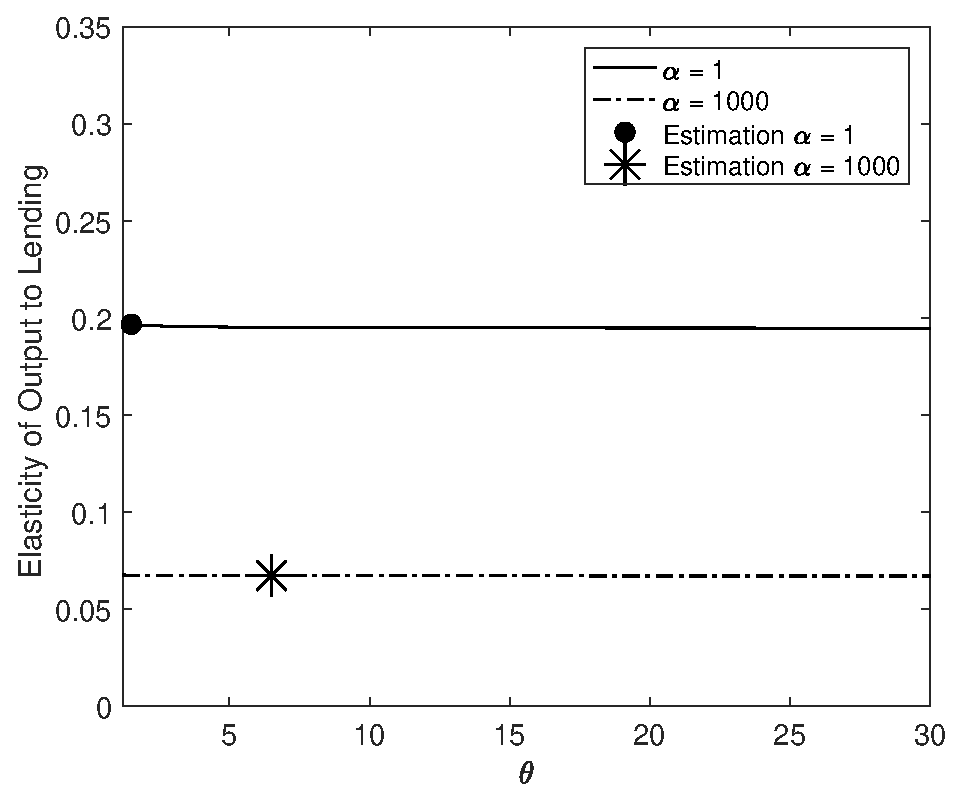
\includegraphics[scale=0.5]{Figures/output_loop_theta.eps}
\end{figure}
\end{frame}



\begin{frame}{Credit dependence and Output}
%\begin{minipage}[t]{0.48\linewidth}
\begin{figure}
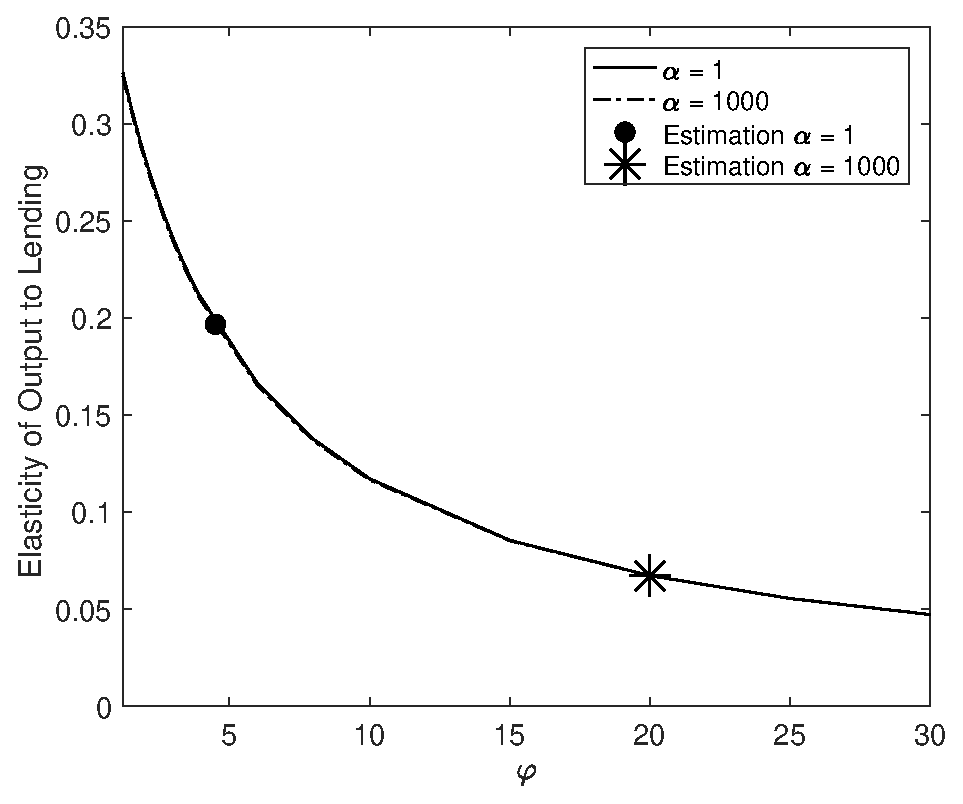
\includegraphics[scale=0.5]{Figures/output_loop_varpsi.eps}
\end{figure}
\end{frame}




\begin{frame}{Result not driven by $\alpha$ itself}
\begin{figure}
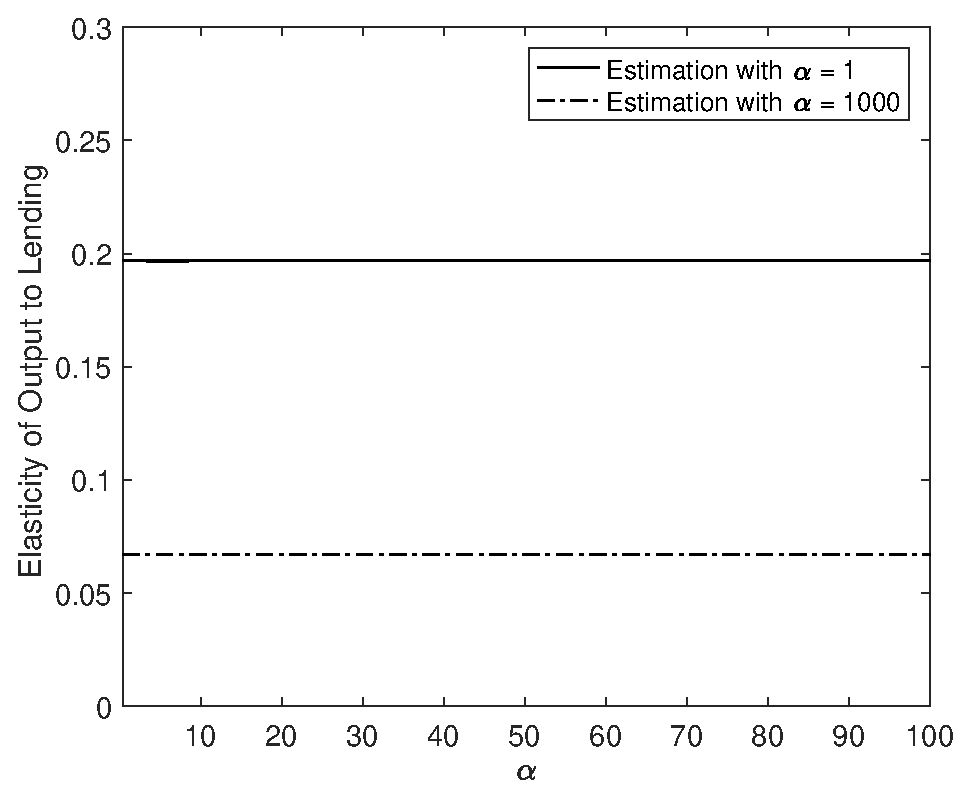
\includegraphics[scale=0.5]{Figures/output_loop_alpha.eps}
\end{figure}
\end{frame}

\begin{frame}{Irrelevance of $\theta$ to an aggregate shock}
\begin{figure}
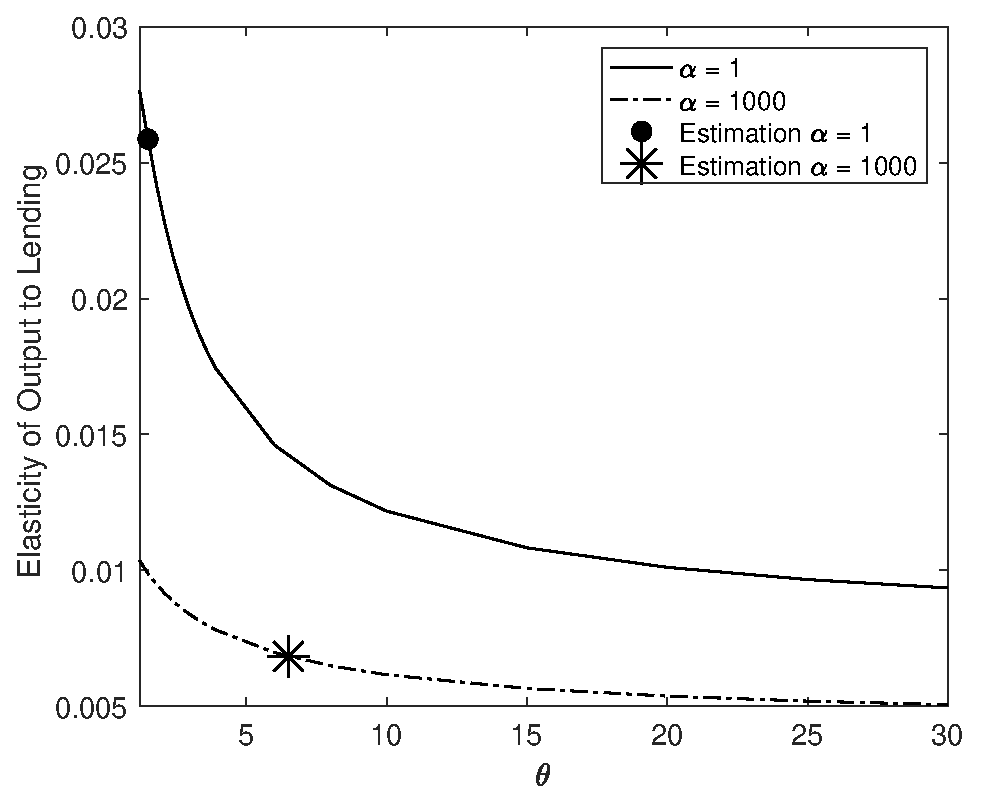
\includegraphics[scale=0.5]{Figures/output_loop_theta_id.eps}
\end{figure}
\end{frame}



\begin{frame}{Credit dependence and Output}
%\begin{minipage}[t]{0.48\linewidth}
\begin{figure}
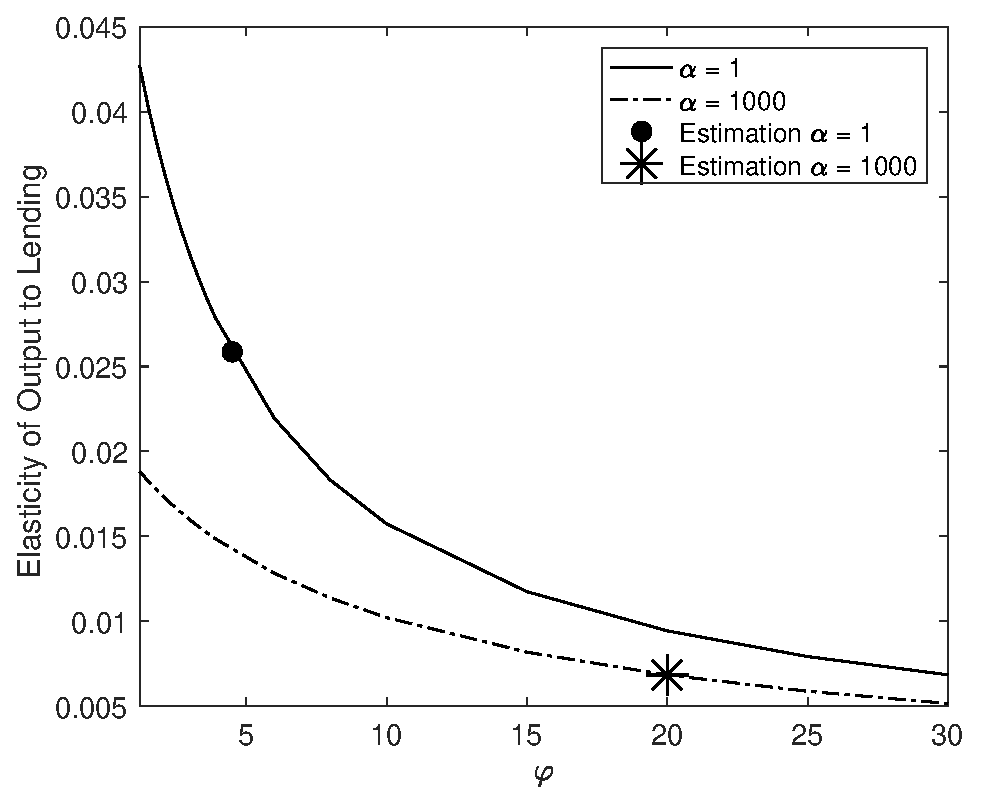
\includegraphics[scale=0.5]{Figures/output_loop_varpsi_id.eps}
\end{figure}
\end{frame}



%
%
%
%\begin{frame}{Aggregate elasticity of output to the shock}
%The results above do not mean that $\theta$ is irrelevant
%\begin{itemize}
%\item For all values of $\theta$ output is as sensitive as lending to the shock
%\item As $\varphi$ increases, output decouples from lending
%\end{itemize}
%Compute the aggregate ``reduced form'' to illustrate this effect
%\begin{align*}
%\varepsilon^{RF} = \frac{\int_0^{\infty} e^{-\rho t} \left(\log(Y_t) - \log(\bar{Y})\right) dt} {\int_0^{\infty} e^{-\rho t} \left( \log(\text{Equity}_t + \bar{\text{Deposits}})  - \log(\bar{\text{Equity}} +\bar{\text{Deposits}})\right) dt}
%\end{align*}
%\end{frame}
%
%
%
%\begin{frame}{The elasticity of aggregate output to bank funding}
%\begin{figure}
%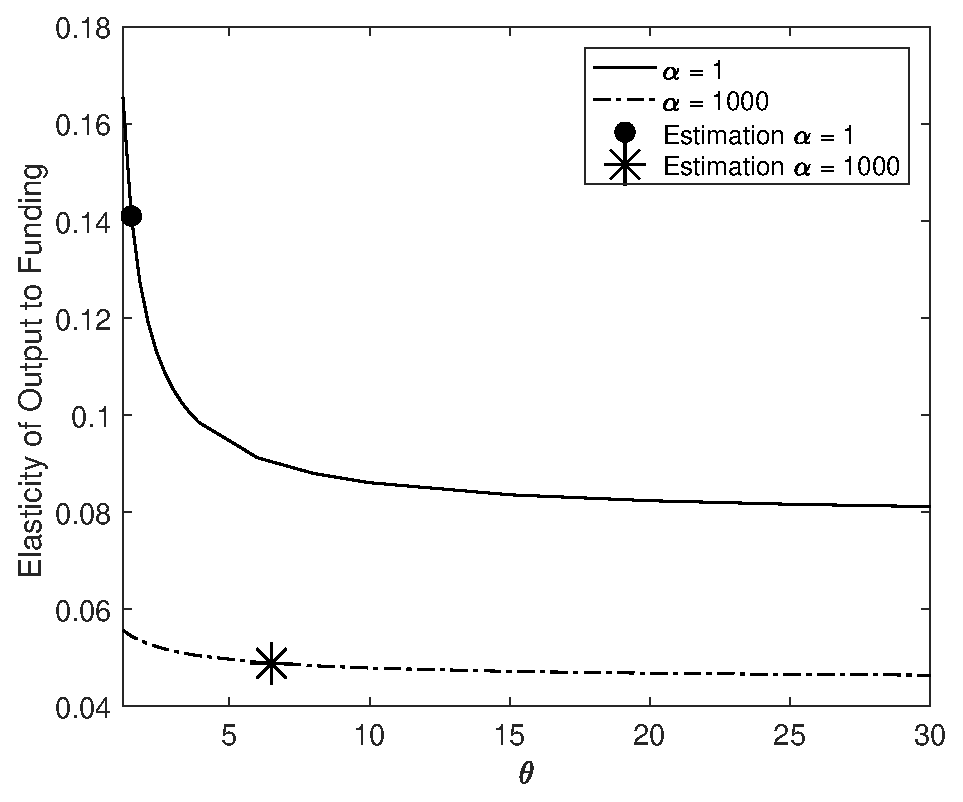
\includegraphics[scale=0.5]{Figures/output_loop_theta2.eps}
%\end{figure}
%\end{frame}
%
%\begin{frame}{The elasticity of aggregate output to bank funding}
%%\begin{minipage}[t]{0.48\linewidth}
%\begin{figure}
%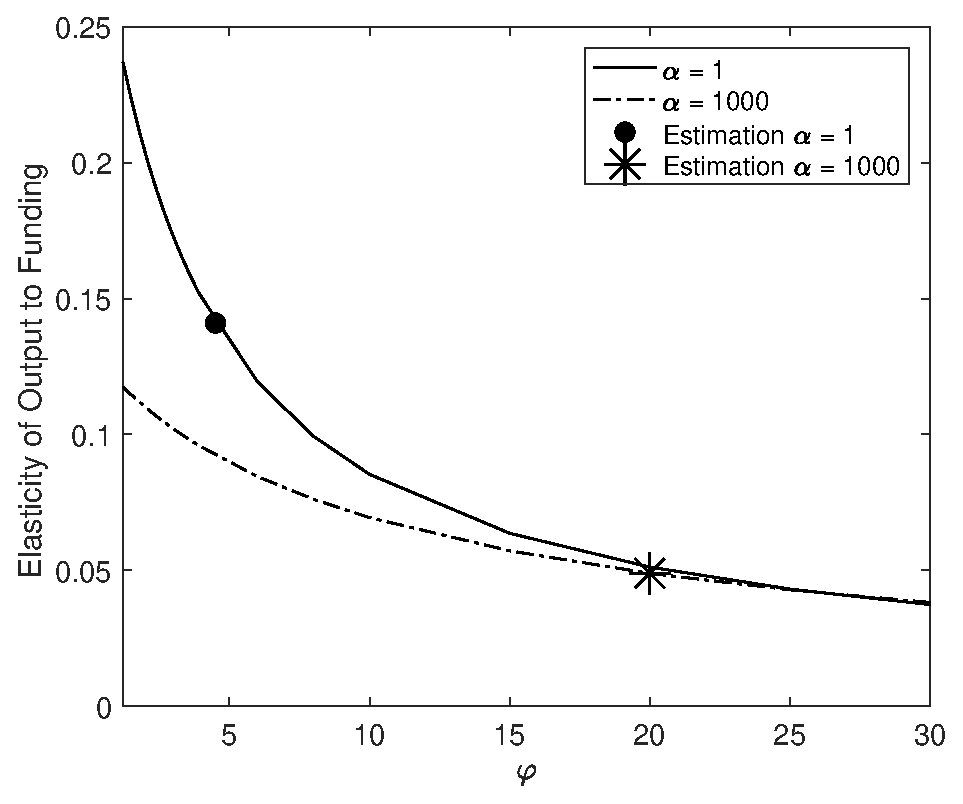
\includegraphics[scale=0.5]{Figures/output_loop_varpsi2.eps}
%\end{figure}
%\end{frame}
%
%
%
%\begin{frame}{Summary}
%\begin{table}
%\begin{tabular}{lcc}
%\hline
%\hline
%Statistic & $\alpha = 1$ & $\alpha = 1000$ \\
%\hline
%Output to Lending (\%) & 19.7 & 6.7 \\
%Output to Funding (\%)  & 14.1 & 4.8 \\
%\hline
%\hline
%\end{tabular}
%\end{table}
%\begin{itemize}
%\item When $\alpha = 1$ effects are three times larger
%\end{itemize}
%\end{frame}

\begin{frame}{Back-of-the-envelope aggregation}
Aggregate the cross-sectional estimates

\begin{align}
\varepsilon^{cs} = \frac{\int_0^T e^{-\rho t} \int_0^1 \left(\log(Y_{jt}) - \log(Y_{ct})\right) dj dt} {\int_0^T e^{-\rho t}   \int_0^1 \log(\text{Lending}_{jt})  - \log(\text{Lending}_{ct}) dj dt}
\end{align}
\end{frame}


\begin{frame}{GE versus PE effects}
\begin{figure}
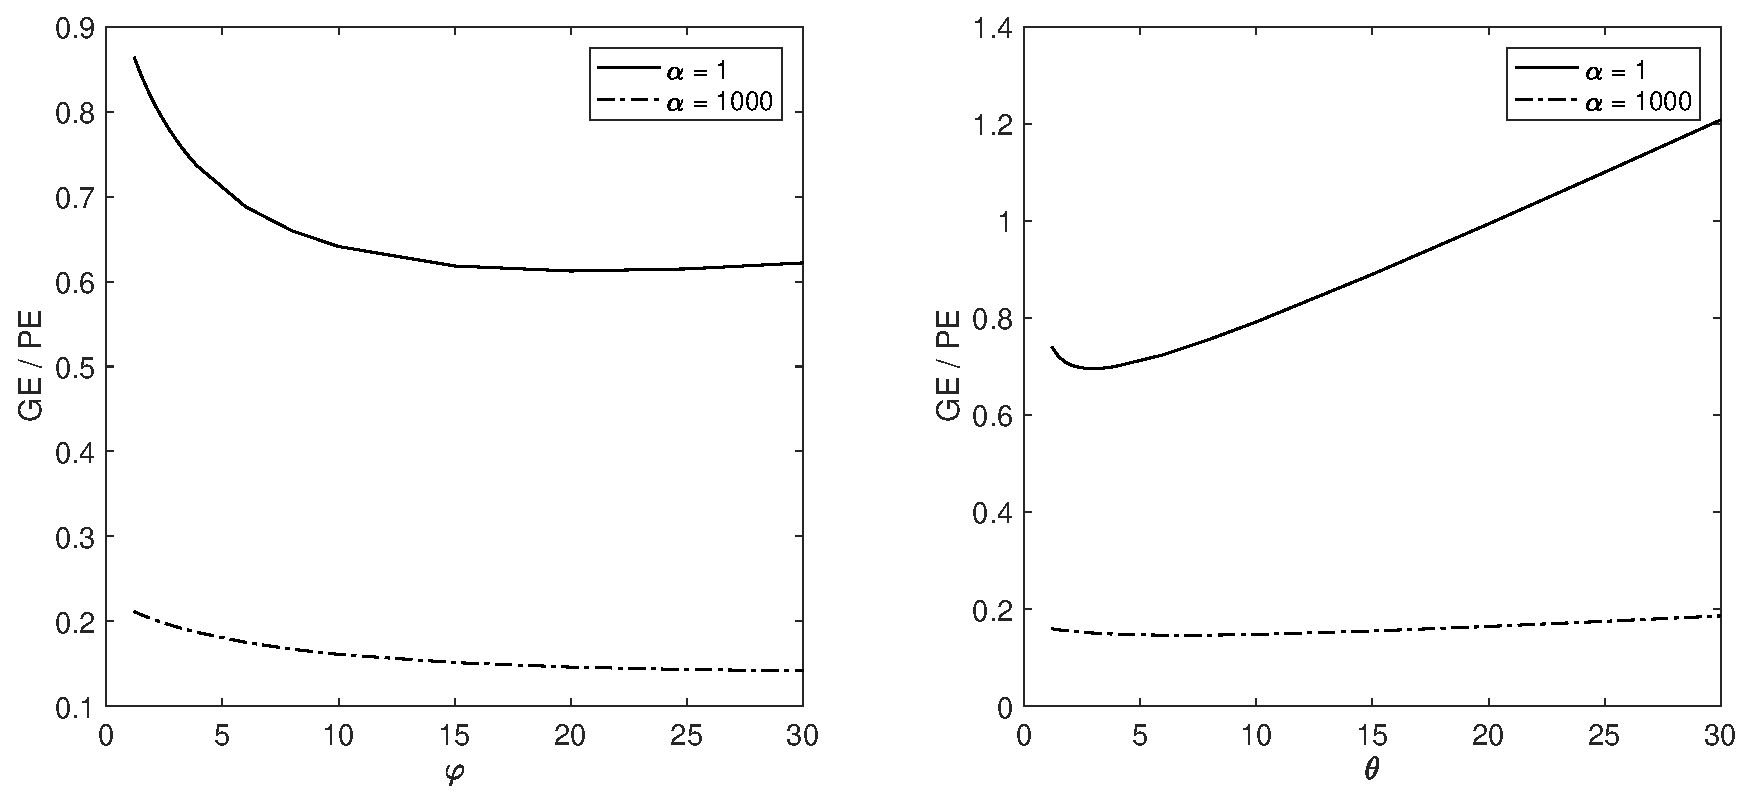
\includegraphics[scale=0.35]{Figures/ge_to_pe_2_varphi_theta.eps}
\caption*{Ratio of GE to PE falls in output after a one-bank shock}
\end{figure}

\end{frame}

%
%
%{  \setbeamercolor{background canvas}{bg=colblue2}
%	\begin{frame}
%		\addtocounter{framenumber}{-1}
%		\thispagestyle{empty}
%		
%		\begin{center}
%			{\Large \color{white} Counterfactuals}
%		\end{center}
%		
%	\end{frame}
%}
%
%
%\begin{frame}{List of counterfactuals}\label{counterfactuals}
%In the paper...
%\begin{itemize}
%\item More competitive banking sector  \hyperlink{more_banks}{\beamerbutton{Go}}
%\item Shock to a more ``distant'' bank  \hyperlink{distant_bank}{\beamerbutton{Go}}
%\item One bank vs. all bank shocks  \hyperlink{all_vs_one}{\beamerbutton{Go}}
%\item Shocks to credit demand (quantitatively different)
%\end{itemize}
%\end{frame}


\begin{frame}{Conclusions}
\begin{itemize}
\item Cross-sectional regressions are informative about aggregate shocks
\begin{itemize}
\item Employment growth on pre-existing exposure
\item  Credit growth on pre-existing exposure
\end{itemize}
\item Firm fixed-effect regressions informative about idiosyncratic shocks
\item Observational equivalence on firm-level regressions
\begin{itemize}
\item GE $\approx$ 70\% PE  (preferred)
\item GE $\approx$ 20\% PE (alternative)
\end{itemize}
\end{itemize}
\end{frame}

\section{Catherine, Chaney, Huang, Sraer, Thesmar (2021)}


\begin{frame}{Motivation}
\begin{itemize}
\item Cross-sectional effects of having more collateral on firm-investment
\item Broad literature of firm excess sensitivity
\item What are the TFP and output effects of collateral constraints?
\end{itemize}
\end{frame}

\begin{frame}{Cross-Sectional Elasticity}
\[ \frac{i_{it}}{k_{it}} = a + \beta \frac{REValue_{it}}{k_{i,t-1}} + Offprice_{it} + \Gamma' X_{it} + \nu_{it}\]
\begin{itemize}
\item Chaney, Sraer, Thesmar (2012) AER paper all about this
\item Exogenous shock to real estate value, increases the value of collateral, which increases debt capacity and investment for financially-constraint firms
\end{itemize}
\end{frame}

\begin{frame}{Production}
\[q_{it} = e^{z_{it}} \left(k_{it}^{\alpha} l_{it}^{1-\alpha}\right)\]
\begin{itemize}
\item Firm-level productivity AR(1)
\item Downward-sloping demand curves
\[q_{it} = Q p_{it}^{-\phi}\]
\item Curvature in the revenues minus wage bill
\[\pi(z_{it},k_{it}) = bQ^{1-\theta} w^{-(1-\alpha)\theta/\alpha} e^{z_{it} \theta/\alpha} k_{it}^{\theta}, \]
\item For $\theta = \frac{\alpha(\phi-1)}{1+\alpha(\phi-1)}$
\item Why is it important?
\end{itemize}
\end{frame}

\begin{frame}{Capital adjustment frictions}
\begin{itemize}
\item Law of motion of capital stock
\[k_{it+1} = k_{it} + i_{it} -\delta k_{it} \]
\item Convex costs of adjustment
\[\frac{c}{2} \left(\frac{i}{k}\right)^2 k \]
\end{itemize}
\end{frame}


\begin{frame}{Financial Frictions}
\begin{itemize}
\item interest rate spread on debt $m$
\item Cost of issuing equity. If cash-flows are $x$, post-issuance
\[G(x) = x(1 + e 1_{x < 0})\]
\item Collateral constraint
\[(1+r) d_{it+1} \leq s((1-\delta) k_{it+1} + \mathbb{E}(p_{t+1}|p_t) \times h)\]
\item $s$ parameterize loose or tight the constraint is
\item $h$ is the amount of real estate (common across firms)
\item Friction comes from limited enforcement
\item $h$ is a parameter
\end{itemize}
\end{frame}

\begin{frame}{Estimation}
\begin{itemize}
\item Autocorrelation of investment rates to infer the adjustment cost $c$
\item This is usual in investment models (see Cooper and Haltiwanger, 2006)
\item Use the cross-sectional elasticity $\beta$ in an SMM to estimate $s$
\item Use data on equity issuances to estimate $e$
\end{itemize}
\end{frame}

\begin{frame}{Capital or Financial frictions?}
\begin{figure}
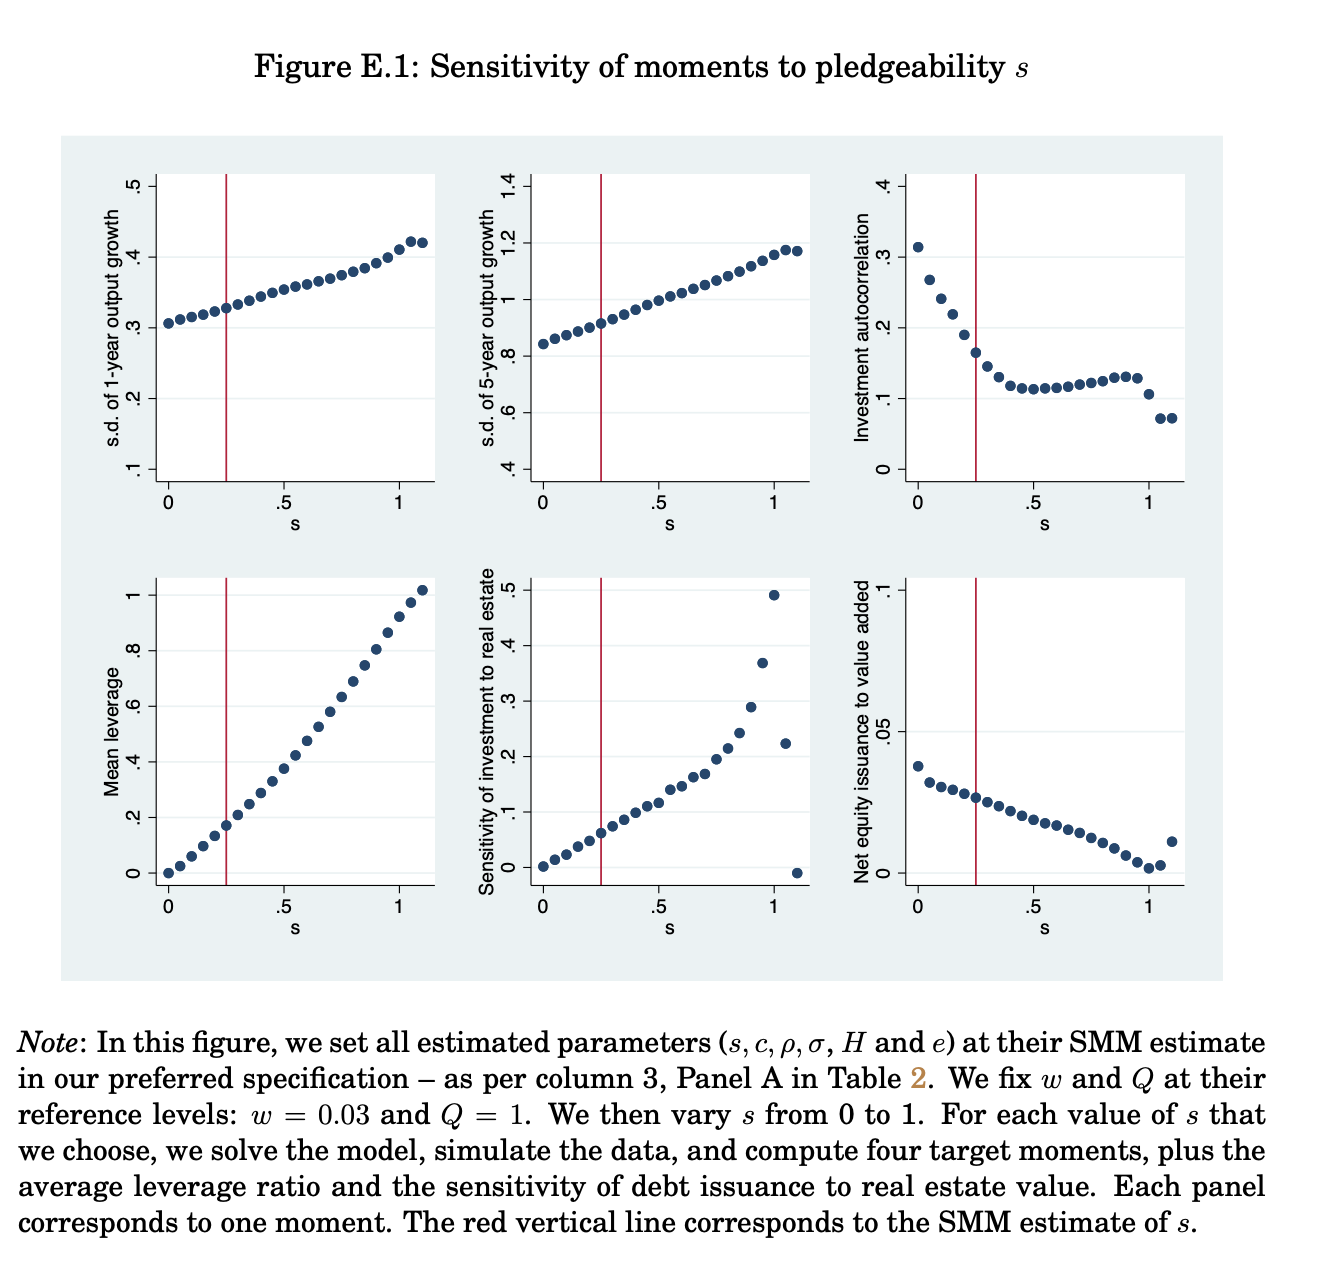
\includegraphics[scale=0.35]{figures/cchst_1}
\end{figure}
\end{frame}

\begin{frame}{Capital or Financial frictions?}
\begin{figure}
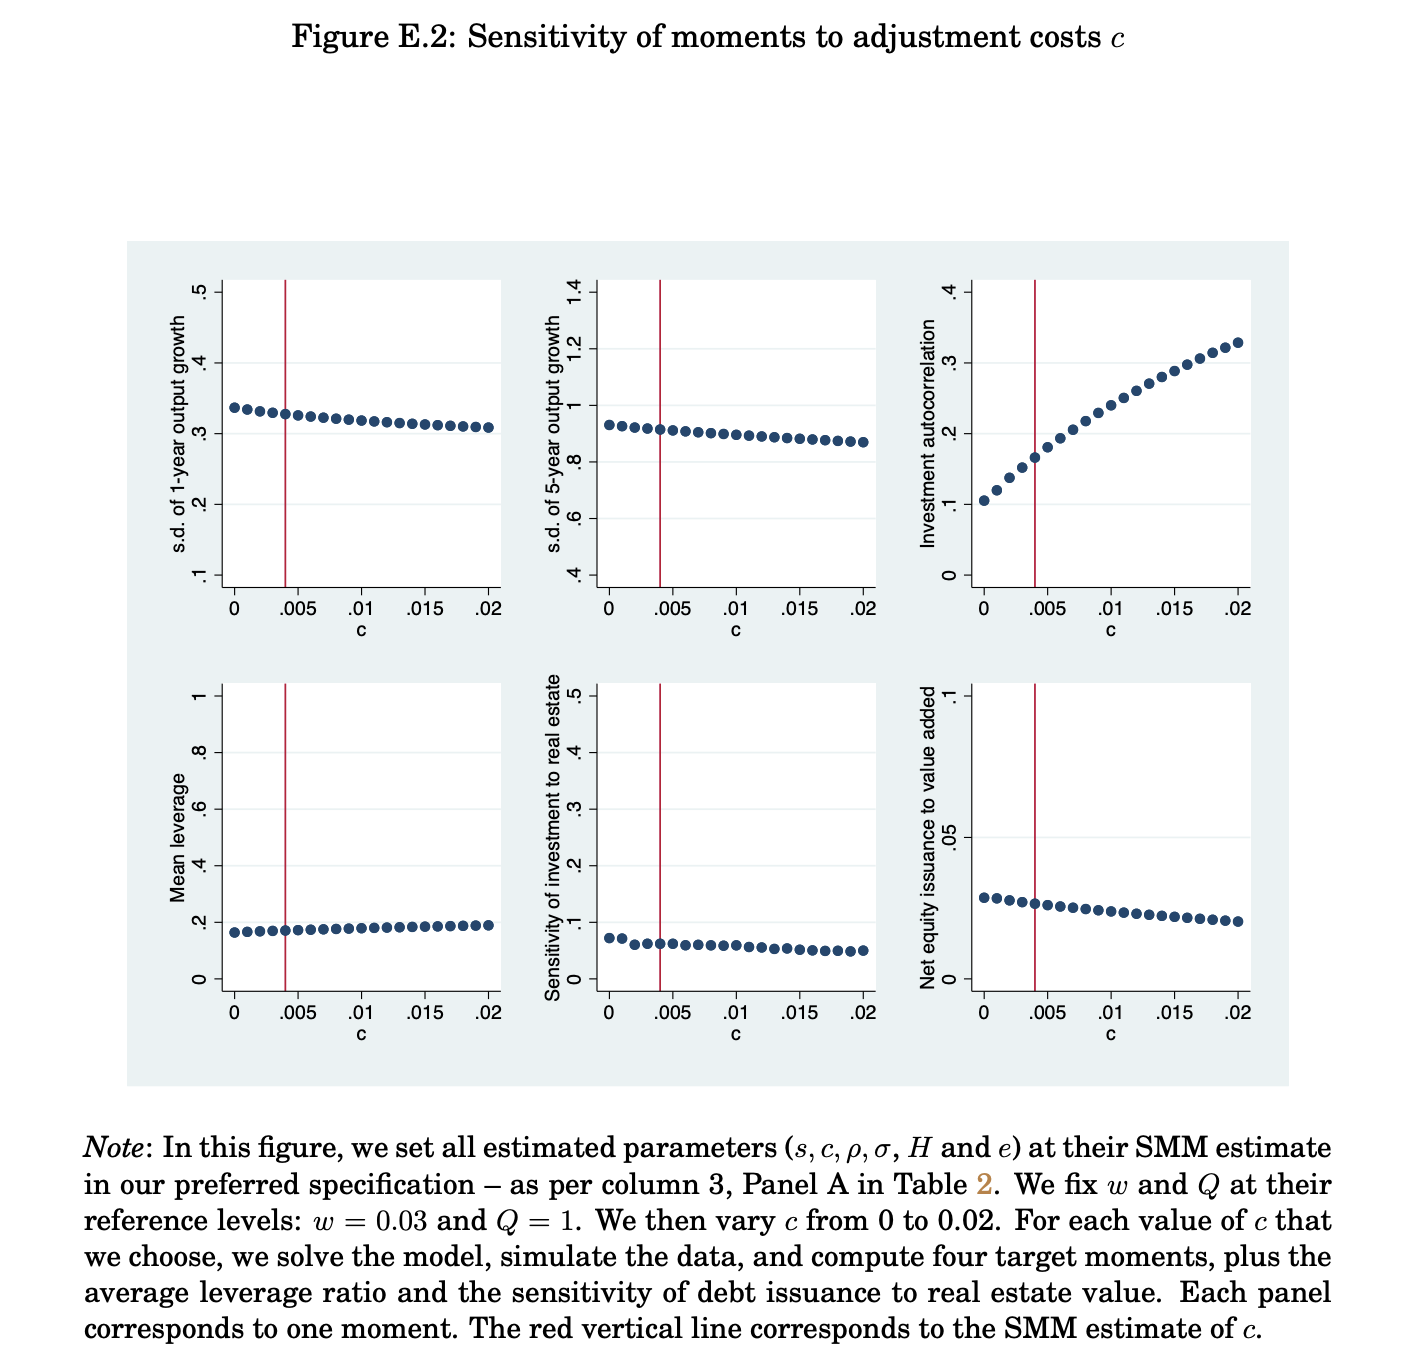
\includegraphics[scale=0.35]{figures/cchst_2}
\end{figure}
\end{frame}

\begin{frame}{GE Block}
\begin{itemize}
\item Aggregate production $Q$ is CES
\item Resource constraint
\[Q_t = C_t + I_t + AC_t\]
\item Quasi linear utility
\[L^s_t = \bar{L} w^{\epsilon}_t\] 
\end{itemize}
\end{frame}

\begin{frame}{Counterfactual}
\begin{itemize}
\item Two alternatives of creating the world with no financial constraints
\begin{enumerate}
\item $s \rightarrow \infty$
\item $e = 0$
\end{enumerate}
\item Which is the correct one?
\end{itemize}
\end{frame}

\begin{frame}{Results}
\begin{figure}
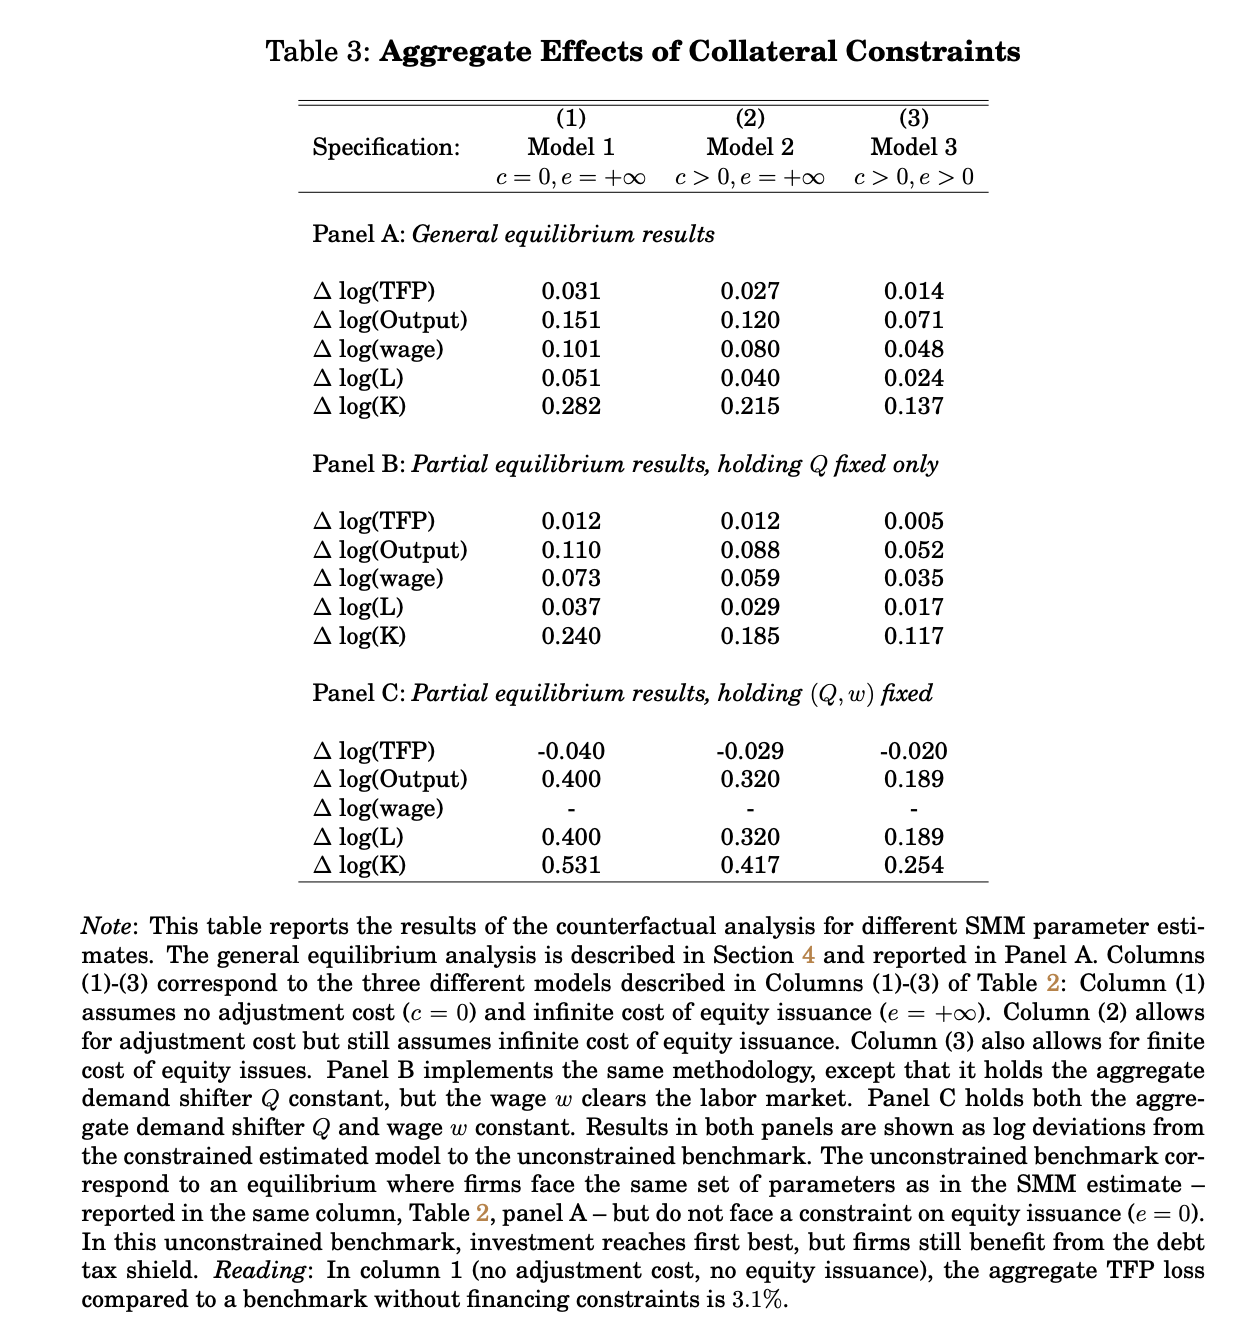
\includegraphics[scale=0.35]{figures/cchst_3}
\end{figure}
\end{frame}

\begin{frame}{Results}
\begin{itemize}
\item The results depend a lot on the persistence of productivity $\rho$
\item Why?
\item Recommended reading: Moll (2014)
\end{itemize}
\end{frame}

\begin{frame}{Mispecification}
\begin{itemize}
\item Two alternatives to estimate the model
\begin{itemize}
\item Estimate the structural parameters $\Theta$ to target (among others) $\beta$
\item Estimate the structural parameters $\Theta$ to target (among others) debt to capital ratios
\end{itemize}
\item Which is better?
\item Offer one metric: Effects of model mispecification
\item Also: Effect of measurement error
\end{itemize}
\end{frame}

\begin{frame}{Mispecification}
\begin{itemize}
\item Idea: Complicate the model
\begin{enumerate}
\item Intangible capital
\item Mismeasured capital
\item Economic depreciation $\neq$ accounting depreciation
\item Secured debt
\end{enumerate}
\item Estimate the extended and restricted (benchmark) model
\item What is the effect on the counterfactuals of TFP and output
\item Follows Isaiah, Gentzkow, Shapiro (2017) (which I should study).
\end{itemize}
\end{frame}

\begin{frame}{Mispecification}
\begin{figure}
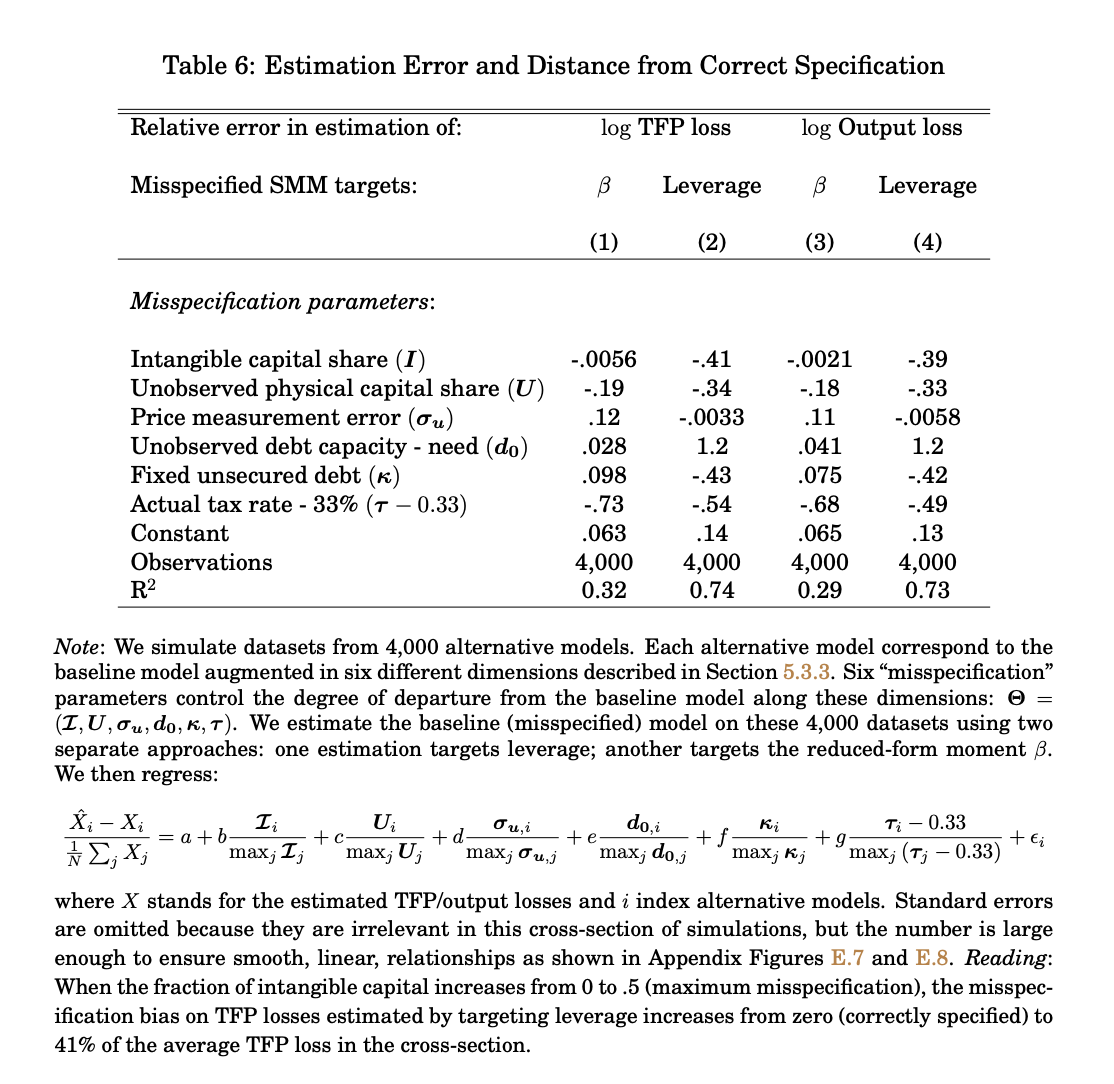
\includegraphics[scale=0.35]{figures/cchst_4}
\end{figure}
\end{frame}



\section{Huber (2022) - Aggregating with Data}

\begin{frame}{Huber (2022)}
\begin{itemize}
\item This discussion follows Huber (2022) ``Estimating General Equilibrium Spillovers of Large-Scale Shocks''
\item Usual method is to aggregate using a model
\item Or to generate a sufficient statistic
\item Potentially could estimate spillovers directly using experiments or quasi-experiments
\end{itemize}
\end{frame}

\begin{frame}{Huber (2022)}
\begin{itemize}
\item There is a treatment that directly affects firms in the treatment
\item But also affects firms that belong to the same ``group'' as treated firms
\item Groups can be industries, regions, supply chains,..
\item Direct spillover estimation requires exogenous treatment across firms \textbf{and} groups
\end{itemize}
\end{frame}

\begin{frame}{Intuition}
\begin{itemize}
\item To estimate the spillover the standard practice is to include leave-out means in the regression
$$y_{fg} = \beta_0 + \beta_1 Treatment_{fg} + \beta_2 \overline{Treatment}_g + \epsilon_{fg}$$
\item where $\overline{Treatment}_g = \frac{1}{N-1} \sum_{j \neq f \in g} y_{jg}$
\item Two complications in estimating $\beta_2$
\begin{enumerate}
\item Multiple types of spillovers
\item Mismeasured treatment status due to nonlinear effects or measurement error
\end{enumerate}
\end{itemize}
\end{frame}


\begin{frame}{Intuition}
\begin{itemize}
\item Imagine a firm $f$ in sector $s$, that produces in region $r$, and sells in region $d$
\item Should the right regression be?
$$y_{fs} = \beta_0 + \beta_1 Treatment_{fs} + \beta_2 \overline{Treatment}_s + \epsilon_{fs}$$
\item or
$$y_{fr} = \beta_0 + \beta_1 Treatment_{fr} + \beta_2 \overline{Treatment}_r + \epsilon_{fr}$$
\item or
$$y_{fd} = \beta_0 + \beta_1 Treatment_{fd} + \beta_2 \overline{Treatment}_d + \epsilon_{fd}$$
\item or all of them $y_{fsrd}$ including all the leave-out means?
\end{itemize}
\end{frame}


\begin{frame}{Setting}
\begin{itemize}
\item Let's consider the setting in Huber (2022)
\[y_i  = \beta	x_i  + \sum_{j\neq i, r(j) = r(i)} \lambda^j x_j + \sum_{ k \neq i, s(k) = s(i)} \gamma^k x_k + \alpha + \epsilon_i\] 
\item here $x$ is treatment status. $s$ are sectors, $r$ are regions.
\item Treatment is as good as random
$$\mathbb{E}(x_i \epsilon_i) = 0 \forall i$$
\item The biases we are talking about will not arise with assignment or reflection problems
\end{itemize}
\end{frame}


\begin{frame}{Setting}
\[y_i  = \beta	x_i  + \sum_{j\neq i, r(j) = r(i)} \lambda^j x_j + \sum_{ k \neq i, s(k) = s(i)} \lambda^k x_k + \alpha + \epsilon_i\] 
\begin{itemize}
\item Assumption: No heterogeneity in spillovers $\lambda^j = \lambda$, and $\gamma^k = \gamma$
\item So outcomes are functions of individual treatment, and two ``leave-out'' means
\[y_i  = \beta	x_i  +  \lambda \overline{x}_{r(i)} + \gamma \overline{x}_{s(i)}  + \alpha + \epsilon_i\] 
\item Treatment status (intensity)
\[x_i = z_i + u_r(i) + u_s(i) + \nu_i \]
\item $z_i$ is observable, uncorrelated within $r$ and $s$, and will be an instrument for $x$
\item $u_r$, $u_s$, $z$, $\nu$ are uncorrelated with each other, and with $\epsilon$
\end{itemize}
\end{frame}

\begin{frame}{Testing for the wrong spillover}
\begin{itemize}
\item Imagine the right DGP is
\[y_i = x_i + \overline{x}_{r(i)} + \epsilon_i\]
\item ($\beta = 1$, $\lambda = 1, \gamma = 0)$
\item Treatment varies systematically across regions and sectors
\item Instead you run the regression
\[y_i = b_1 x_i + b_2 \overline{x}_{s(i)} + \xi_i\]
\item $\hat{b}_2/\hat{b}_1 = -0.33$.
\item Why? $\overline{x}_{r(i)}$ enters the error term 
\item $\overline{x}_{r(i)}$ is correlated with $u_r(i)$, and therefore with $x_i$
\item Biases both $\hat{b}_1$ and $\hat{b}_2$
\end{itemize}
\end{frame}

\begin{frame}{Solution}
\begin{itemize}
\item Economic theory!
\item Example of Mian and Sufi: regional spillovers should be mostly (only?) important for non-tradeable firms
\item Test $H_0$ of zero regional spillovers among tradeable firms
\item Other solution, use $\bar{z}_s$, $\bar{z}_s$ as instruments
\end{itemize}
\end{frame}


\begin{frame}{Testing for the incorrect spillover}
\begin{figure}
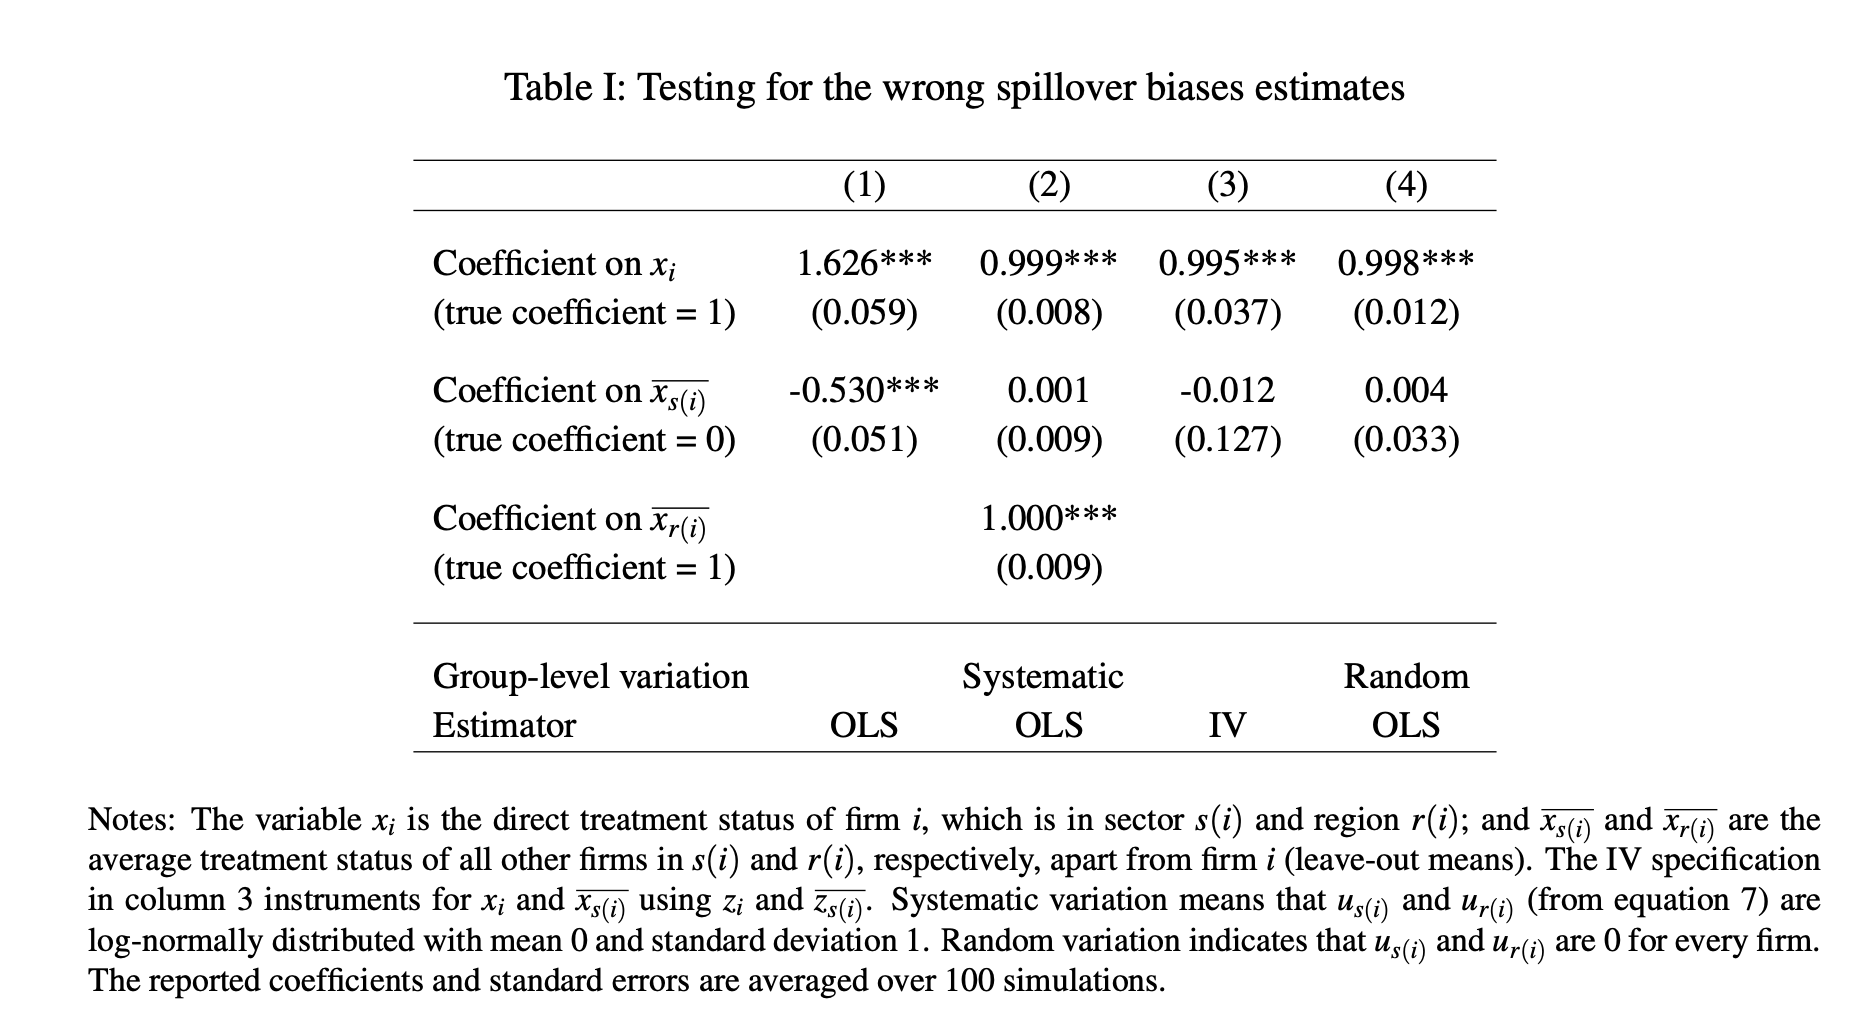
\includegraphics[scale=0.35]{figures/h_ge_6}
\end{figure}
\end{frame}



\begin{frame}{Testing for incomplete spillovers}
\begin{itemize}
\item Imagine the right DGP is
\[y_i = x_i + \overline{x}_{r(i)} + \overline{x}_{s(i)} \epsilon_i\]
\item ($\beta = 1$, $\lambda = 1, \gamma = 1)$
\item Treatment varies systematically across regions and sectors
\item Instead you run the regression
\[y_i = b_1 x_i + b_2 \overline{x}_{s(i)} + \xi_i\]
\end{itemize}
\end{frame}


\begin{frame}{Testing for the incorrect spillover}
\begin{figure}
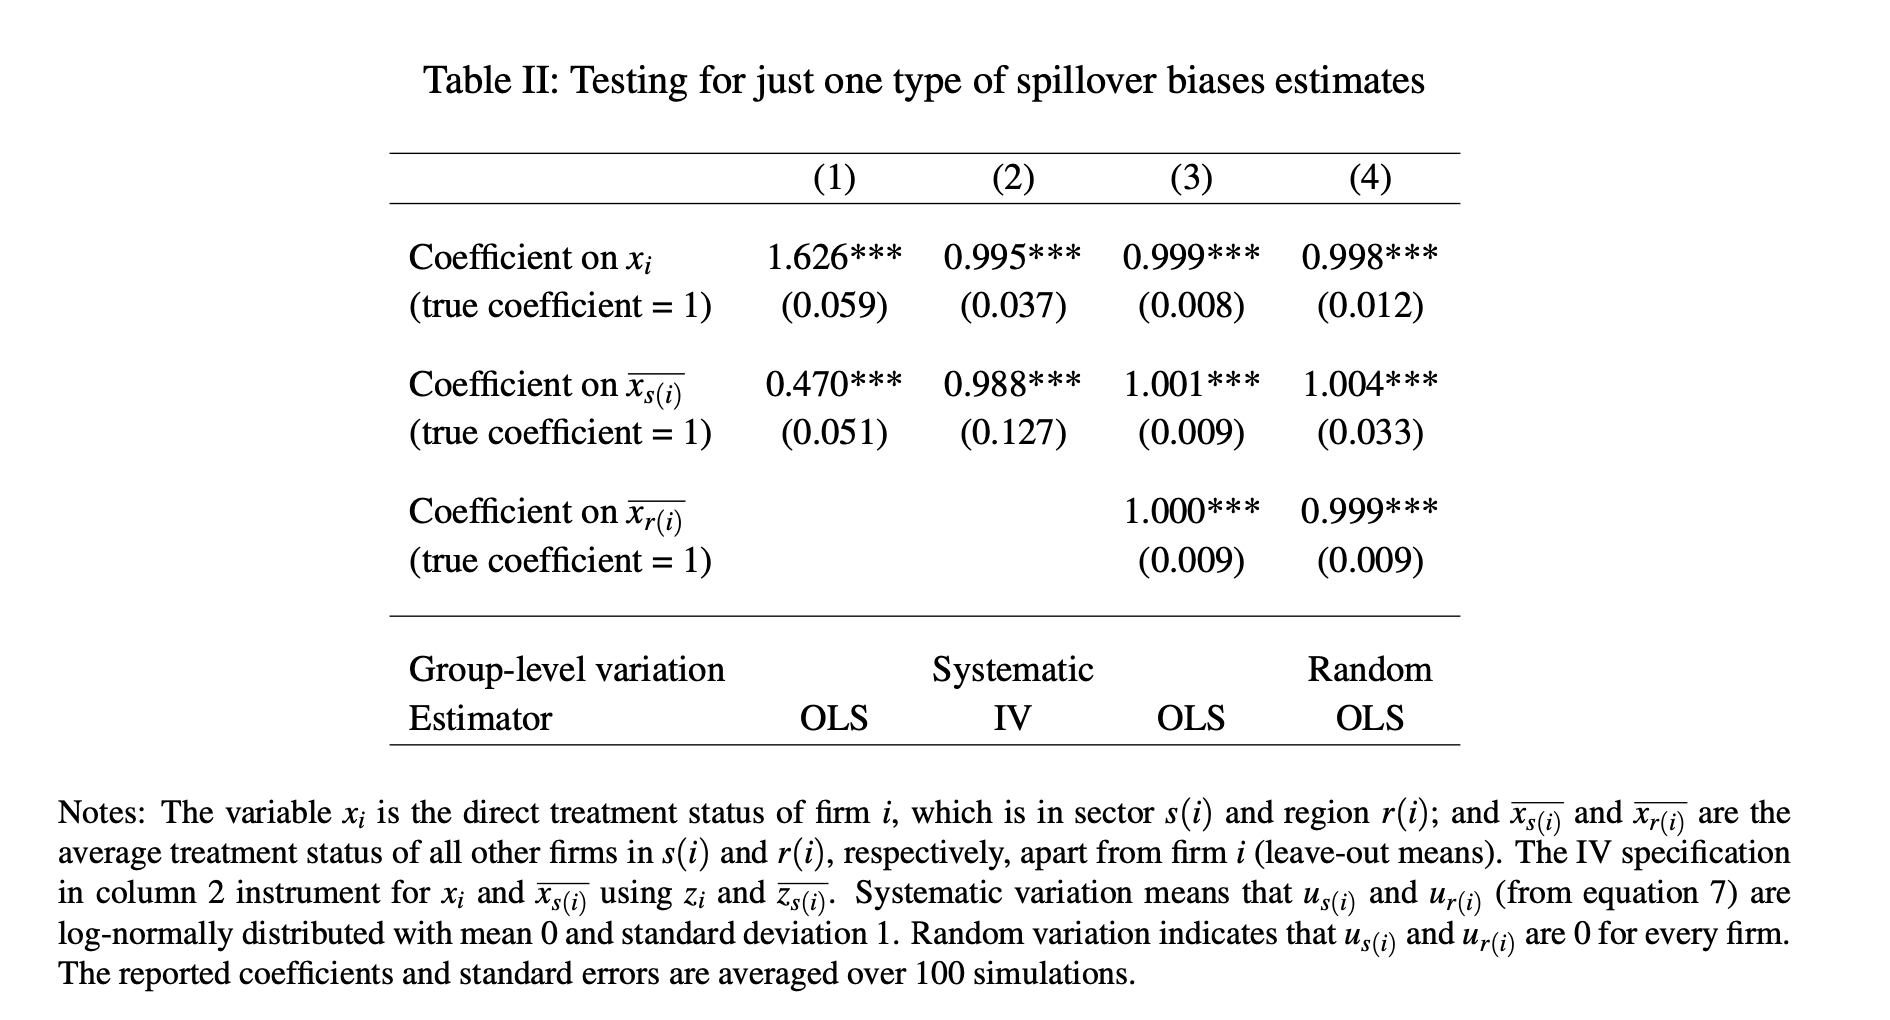
\includegraphics[scale=0.35]{figures/h_ge_7}
\end{figure}
\end{frame}

\begin{frame}{Measurement Error}
\begin{itemize}
\item You observe $x^*_i = x_i + \eta_i$
\item $\eta$ uncorrelated with $\epsilon, z, u_r, u_s,\nu$
\item The most benign case of measurement error
\item In this case $\overline{x}^*_{r(i)} = \overline{x}_{r(i)} + \overline{\eta}_{r(i)}$
\item Intuitively, variation caused to $x$ will be attributed to $\overline{x}$
\item You should think carefully about measurement error
\end{itemize}
\end{frame}


\begin{frame}{Measurement Error without True Spillovers}
\begin{figure}
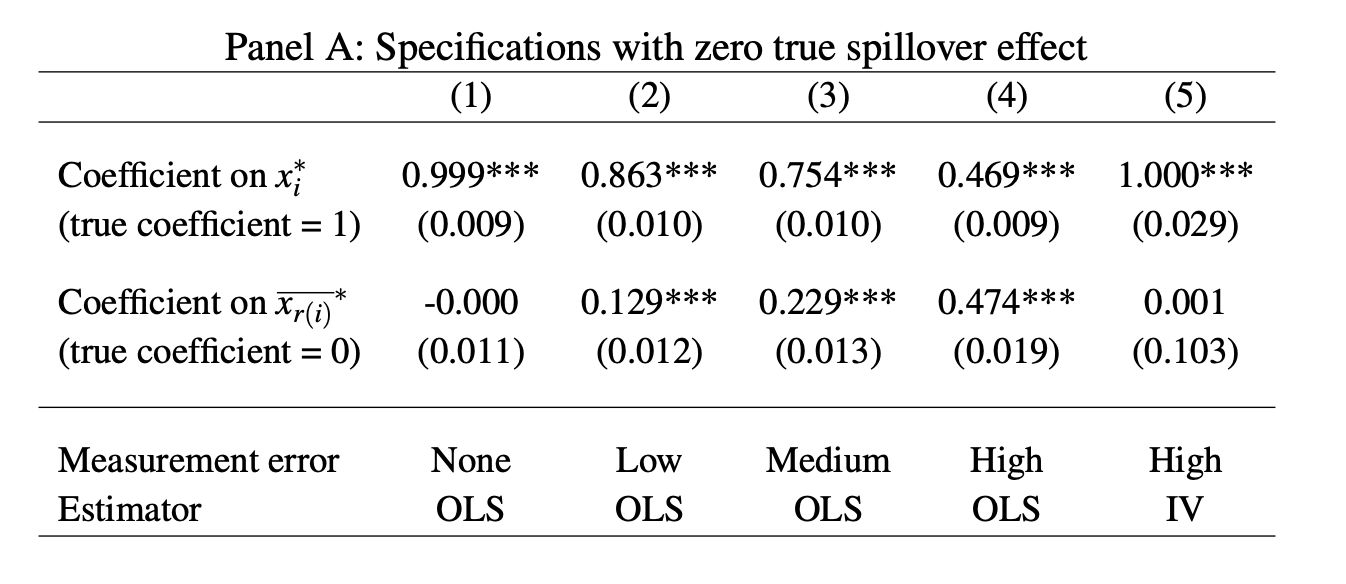
\includegraphics[scale=0.35]{figures/h_ge_1}\\
Instrument $x$ and $\bar{x}$ with $z$ and $\bar{z}$.
\end{figure}
\end{frame}

\begin{frame}{Measurement Error with True Spillovers}
\begin{figure}
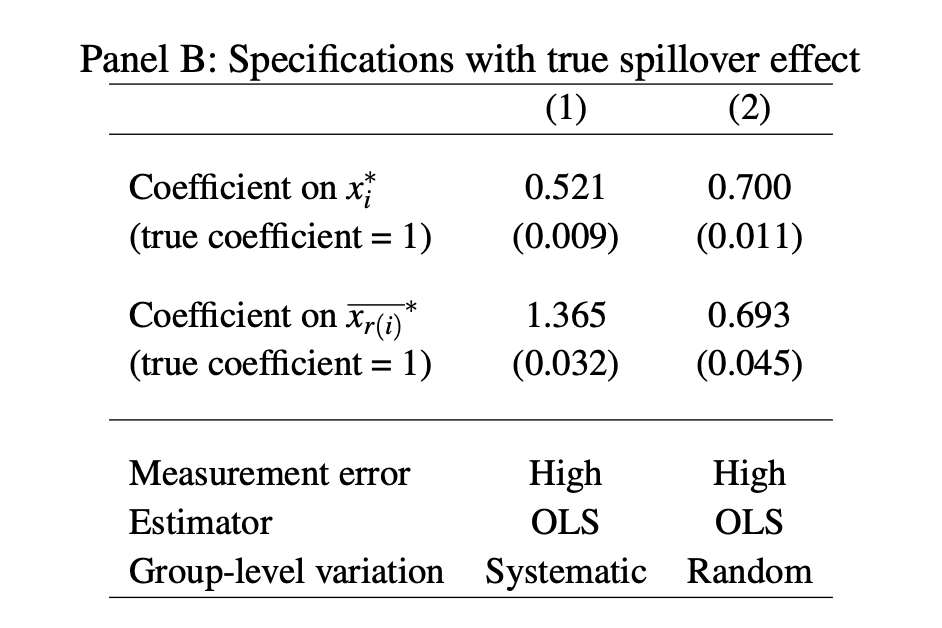
\includegraphics[scale=0.35]{figures/h_ge_2}\\
 \end{figure}
 Spillover over or under estimated depending on whether $u_r$ changes across regions. Similar issues in peer-effect literature in labor (Ammermueller and Pischke (2009).
\end{frame}


\end{document}

